\documentclass[german,version-2020-11]{uzl-thesis}
% !TeX program = lualatex

\UzLThesisSetup{
  Logo-Dateiname        = {institutslogo.pdf},
  Verfasst              = {am}{Institut für Informationssysteme},
  Titel auf Deutsch = { Evaluation eines Algorithmus zur Absicherung von Datenbanken vor probabilistischer Inferenz},
  Titel auf Englisch = { Evaluation of an Algorithm for Securing Databases from Probabilistic Inference},
  Autor                 = {Kevin Schmelzer},
  Betreuerin            = {Prof. Dr. Ralf Möller},
  Mit Unterstützung von = {Simon Schiff},
  Bachelorarbeit,
  Studiengang           = {IT-Sicherheit},
  Datum                 = {18. August 2020},
  Abstract              = {
   The confidentiality of sensitive data requires special protection, especialy in the medical area, where dealing with patients data. For this purpose, access-control are used to deny requests to sensitive data. However, these mechanisms do not be aware of that by combining statistcal information and results of smart chosen queries on non-sensitve data, information on sensitive data can still be inferred. One solution to prevent an attacker from inferring sensitive data is the Database Inference Control (DBIC). A DBIC mechanism is the prototype Angerona, which uses definitions of probabilistic dependency rules to deny access to sensitive data. In this work, Angerona is evaluated, since it has not yet been empirically evaluated on real data. This will be done by  test the security and runtime on real medical data. It was determined, that the runtime is possible for real world use cases, it takes too long to answer queries to be used in practice.
  },
  Zusammenfassung       = {
  	Die Vertraulichkeit sensibler Daten erfordert einen besonderen Schutz, insbesondere im medizinischen Bereich, in dem mit Patientendaten gearbeitet wird. Dafür werden Zugangskontrollmechanismen verwendet, um Anfragen an sensible Daten zu verweigern. Diese Mechanismen beachten jedoch nicht, dass durch Kombinierung von statistischen Auswertungen und Ergebnisse klug gewählter Anfragen auf unsensible Daten, trotzdem Informationen zu sensiblen Daten hergeleitet werden können. Eine Lösung, um zu verhindern, dass ein Angreifer auf sensible Daten schließen kann, ist die Database Inference Control (DBIC). Ein DBIC-Mechanismus ist der Prototyp Angerona, der anhand von Definitionen von probabilistischen Abhängigkeitsregeln, den Zugriff auf sensible Daten verweigert. In dieser Arbeit wird Angerona evaluiert, da dieser bisher  noch nicht auf echten Daten empirisch evaluiert wurde. Dafür wird, mit echten medizinischen Daten, die Sicherheit getestet und die Laufzeit gemessen. Dabei wurde festgestellt, dass die Laufzeit für praxisnahe Anwendungsfälle zwar möglich ist, jedoch das Beantworten von Anfragen zu lange dauert, um in der Praxis verwendet zu werden.
  },
  %Alphabetische Bibliographie
  % Alternatively:
   Numerische Bibliographie
}

\UzLStyle{pagella basic design}


% Now, include the package you need here using \usepackage. 
\usepackage{dcolumn}
\usepackage{booktabs}
\usepackage{tikz}
\usepackage{biblatex}
\usepackage{cleveref}
\usepackage{caption}
\usepackage{subcaption}
\usepackage{MnSymbol}
\usepackage{algorithmicx}
\usepackage{algorithm}
\usepackage[noend]{algpseudocode}
\usepackage{mathtools }
\usepackage{lscape}
\usetikzlibrary{positioning,shapes,arrows}

\newcolumntype{M}[1]{D{.}{.}{1.#1}}

\addbibresource{thesis.bib}
\begin{document}
\chapter{Einleitung}
Der Schutz von sensiblen Daten ist für viele Unternehmen und andere Einrichtungen wichtig, die persönliche Daten, wie Herkunft, Religion, Alter etc., erfassen, verarbeiten und speichern. Die Relevanz des Themas Privatsphäre und Digitalisierung ist spätestens seit der Wirksamkeit der Europäischen Datenschutz-Grundverordnung (DSGVO) \cite{1} im  Mai 2018 bemerkbar, da die dadurch entstandenen Herausforderungen auf Unternehmensseite diese vor rechtliche und insbesondere auch technische Probleme stellt, weshalb DSGVO-konforme Software-Lösungen entwickelt wurden, um die Arbeit zu erleichtern \cite{9}.\\ 
In dieser Arbeit wird ein besonderer Fokus auf die Privatsphäre in Krankenhäusern gelegt, da in Krankenhäusern viele sensible und persönliche Daten über Patienten erfasst werden. Dabei gab es schon vor der Einführung der DSGVO eine andere Regelung zum Schutz der Privatsphäre speziell im medizinischen Bereich und zwar die Health Insurance Portability and Accountability (HIPAA) aus dem Jahr 1996, aus den USA. Hierbei wird für jeden, der Gesundheitsdaten verarbeitet oder speichert, durch Anordnungen und Regelungen zur Verarbeitung von Daten vorgeschrieben, die Vertraulichkeit der Daten der Patienten durch z.B. Zugangskontrolle, Anonymisierung, richtige Datenspeicherung etc. zu schützen \cite{7}.\\
Bisher wurde die Vertraulichkeit von sensiblen Daten geschützt, indem der Zugang durch Zugangskontrollmechanismen verboten wurde \cite{2}. Jedoch existieren noch weitere Möglichkeiten, um Informationen zu sensiblen Daten zu erhalten. Daher erfordert der Schutz der Vertraulichkeit von sensiblen Daten einen Schutz vor direktem und indirektem Zugriff auf eine Datenbank. Der direkte Zugriff beschreibt dabei den Zugang zu Daten aus einer Datenbank und wird durch Zugangskontrollen geschützt, indem Zugriffsrechte auf bestimmte Daten oder Tabellen gewährt werden. Beim indirekten Zugriff hingegen, wird versucht, durch statistische Auswertungen von externen Informationen und klug gewählten Anfragen an die Datenbank, an sensible Daten zu kommen. Um den indirekten Zugriff zu verhindern gibt es einige neue Ansätze und eine davon ist die Database Inference Control (DBIC) \cite{22}. Der DBIC-Mechanismus, der in dieser Arbeit evaluiert wird, ist Angerona, wovon erstmals nur ein Prototyp existiert. \cite{guarnieri2017securing} \\ 
Der DBIC-Mechanismus Angerona sichert die Datenbank ab, indem eine probabilistische logische Programmiersprache (\texttt{Problog}) verwendet wird, um das Vorwissen eines Angreifers darzustellen. Dafür wird die Sprache \texttt{ATKLOG} entwickelt, die auf \texttt{Problog} basiert und durch probabilistische Abhängigkeitsregeln das initiale Vorwissen des Angreifers modelliert. Ein Angreifermodell wird benötigt, um das initiale Vorwissen von jedem Benutzer zu speichern.  Um ein Datenbankmodell nach Angerona zu übertragen, werden zuerst alle probabilistischen Abhängigkeitsregeln in ein Bayes-Netz modelliert. Anschließend wird aus dem Bayes-Netz ein Angreifermodell erstellt. Mithilfe von Sicherheitsregeln wird dann ein Schwellwert definiert, der den Zugang zum Datenbanksystem nur zulässt, wenn das Vorwissen des Angreifers unter dem Schwellwert liegt. Dabei wird das Vorwissen während der Interaktion mit Angerona kontinuierlich erweitert alle getätigten Anfragen eines Benutzers in einer Historie gespeichert. \\  
Damit DBIC-Mechanismen, wie Angerona, auch effektiv den indirekten Zugang schützen, müssen diese eine große Menge von probabilistischen Abhängigkeiten abdecken können, um viele verschiedene Angreifermodelle darzustellen und es muss eine angemessene Laufzeit aufweisen, um diese auch auf reale und große Datenbanken anwenden zu können.\\
Die Laufzeit wird dabei in Online- und Offlinelaufzeiten unterteilt, wobei die Onlinelaufzeit  das Intervall zwischen dem Start der Anfrage und der Antwort ist und die Offlinelaufzeit  vom Start des Systems bis das System bereit für eine Eingabe ist. \\
Der Unterschied zu bisherigen DBIC-Mechanismen zu Angerona ist, dass die bisher nur eine begrenzte Anzahl von probabilistischen Abhängigkeiten erlaubt haben und somit nicht für reale Datenbanken tauglich sind. Angerona hingegen soll auch bei komplexen probabilistischen Abhängigkeiten eine angemessene Laufzeit haben und somit in der Praxis nutzbar sein \cite{guarnieri2017securing}. \\

\section{Beiträge dieser Arbeit}
In dieser Arbeit wird ein Verfahren vorgestellt, dass ein Bayes-Netz aus einem Datenbankmodell erstellt und in ein Angreifermodell aus \texttt{ATKLOG} überträgt und es somit mit Angerona ausführbar macht. Außerdem werden die Datenbanken MIMIC-III und eICU für die Krankheit Krebs durch Angerona abgesichert und gezeigt, dass für das MIMIC-III-Beispiel eine Offlinelaufzeit von $77$ Minuten und für eICU $89$ Minuten und die Onlinelaufzeiten für MIMIC-III $36.4$ Sekunden und für eICU $23.6$ Sekunden beträgt und somit nicht effektiv in der Praxis angewendet werden kann. Anschließend wird gezeigt, inwiefern sich die Größe der zu initialisierenden Datenbank, die Komplexität und Größe vom Angreifermodell und die Anzahl der definierten Sicherheitsregeln auf die Offline- und Onlinelaufzeit auswirkt.

\section{Verwandte Arbeiten}
Es gibt einige Ansätze die auch implementierte DBIC-Mechanismen evaluiert haben und zum Ergebnis gekommen sind, dass diese sicher und effizient sind, jedoch waren diese nicht für reale Anwendungsfälle geeignet, weil sie entweder eine zu lange Laufzeit hatten für skalierbare echte Anwendungsfälle oder zu wenig probabilistische Abhängigkeiten unterstützten. \cite{24,guarnieri2017securing} . \\ 
Außerdem unterstützen die meisten DBIC-Mechanismen keine probabilistische Abhängigkeiten sondern nur einfache funktionale Abhängigkeiten und wenn diese probabilistische Abhängigkeiten unterstützten, dann nur eine begrenzte Anzahl. Angerona hingegen unterstützt eine beliebige Größe von probabilistischen Abhängigkeiten.\cite{guarnieri2017securing}

\section{Aufbau dieser Arbeit}
% Replace the following by one or two paragraphs describing the
% thesis's structure.
In \cref{chap:Grundlagen} wird die Funktionsweise von Angerona beschrieben und aus einem Bayes-Netz ein Angreifermodell modelliert und mit Angerona initialisiert. Anschließend werden in  \cref{chap:Modellierung} die genutzten pseudonymisierten und synthetischen Datenbanken vorgestellt und dazu geeignete Angreifermodelle modelliert. Zum Schluss wird in \cref{chap:Auswertung} die Sicherheit und die Online- und Offlinelaufzeit von Angerona geprüft und Kriterien analysiert, die sich auf die Laufzeit auswirken.

\chapter{Grundlagen von Angerona}\label{chap:Grundlagen}
\section{Grundlegendes}
\subsection{Systemmodell}
\begin{figure}[ht]
	\centering
	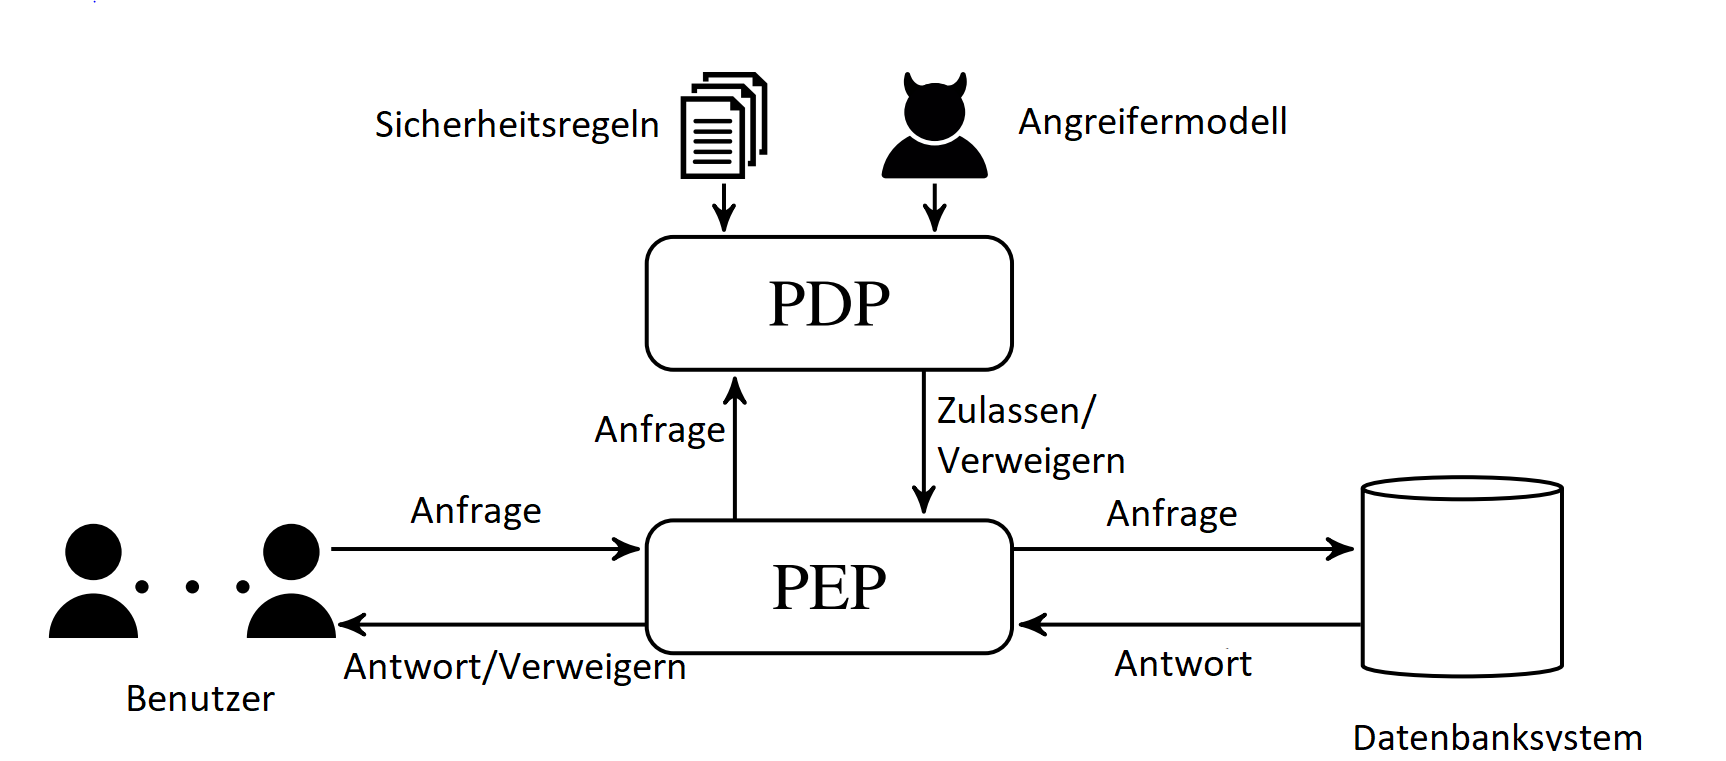
\includegraphics[width=0.9\textwidth]{System-model.PNG}
	\caption{Systemmodell}
	\label{fig1}
\end{figure}
\noindent 
\autoref{fig1} zeigt das von Angerona genutzte Systemmodell. Dabei interagiert der Benutzer mit dem Inferenzkontrollsystem, welches aus den zwei Komponenten Policy Decision Point (PDP) und dem Policy Enforcement Point (PEP) besteht. Das Inferenzkontrollsystem entscheidet anhand von vordefinierten Sicherheitsregeln und einem Angreifermodell, ob die Anfrage des Benutzers an das Datenbanksystem übergeben wird. Dabei wird davon ausgegangen, dass alle Anfragen und Antworten aus dem Systemmodell über sichere Kommunikationskanäle laufen. Außerdem gilt als Voraussetzung, dass jeder Benutzer das Datenbankschema und die Sicherheitsregeln kennt. \\ \\ 
\textbf{Datenbanksystem} Das Datenbanksystem verwaltet alle Daten und antwortet auf Anfragen, um die Daten auszugeben. \\
\textbf{Benutzer} Jeder Benutzer hat ein eigenes Konto um Informationen zu erhalten, indem \texttt{SELECT} Anfragen an das Inferenzkontrollsystem gestellt werden. Dabei hat jeder Benutzer nur Leserechte und kann somit den Datenbankzustand nicht verändern. Jede Anfrage wird vom Inferenzkontrollsystem geprüft und nur ausgeführt, wenn diese von den Sicherheitsregeln autorisiert wird. \\ 
\textbf{Sicherheitsregeln} Die Sicherheitsregeln bestehen aus einer Menge von Regeln, die definieren, welche Informationen geheim gehalten werden sollen. Diese Regeln definieren die Erwartungen jedes Benutzers über den Inhalt der Datenbank als Wahrscheinlichkeitsverteilung. Die Regeln werden formalisiert durch ein Kommando in der Form \texttt{SECRET $q$ FOR $u$ THRESHOLD $l$}, wobei $q$ die Anfrage, $u$ den Benutzer und $l$ den Grenzwert darstellt, bei der die Anfrage genehmigt werden darf,mit $0 \leq l \leq 1$. Eine Sicherheitsregel \enquote{Der Benutzer $u$ ist nicht autorisiert die Antwort von der Anfrage $q$ zu erfahren} wird ausgedrückt mit \texttt{SECRET $q$ FOR $u$ THRESHOLD 1}. Außerdem kann die Regel \enquote{Für alle Benutzer $u \notin \{u_1,\dots,u_n\}$, muss die Erwartung von $u$ bei der Anfrage $q$ kleiner als $l$ sein} mit dem Kommando \enquote{\texttt{SECRET $q$ FOR USERS NOT IN $\{u_1,\dots,u_n\}$ THRESHOLD l}} ausgedrückt werden.\\ 
\textbf{Angreifer} Ein potentieller Angreifer ist jeder Benutzer des Datenbanksystems mit einem Benutzerkonto. Das Ziel eines Angreifers ist es, die Sicherheitsregeln zu verletzen, indem er mindestens auf ein \texttt{SECRET $q$} schließen kann, mit einer Wahrscheinlichkeit unter dem dazugehörigen \texttt{THRESHOLD $l$}. \\ Der Angreifer interagiert mit dem Inferenzkontrollsystem, indem er Anfragen stellt und somit neue Informationen aus den Antworten erhält und Daten, die in Beziehung zueinander stehen , feststellen kann. Ein Beispiel für eine Beziehung zwischen Daten ist zum Beispiel, wenn ein Patient raucht, dass die Wahrscheinlichkeit für Krebs für ihn erhöht ist.  \\
\textbf{Datenbankzustand} Der Datenbankzustand beschreibt die Belegung der Datenelemente in der Datenbank. \\
\textbf{Angreifermodell} Das Angreifermodell definiert das Vorwissen des Benutzers über den aktuellen Datenbankzustand. Im Angreifermodell werden auch die probabilistischen Abhängigkeitsregeln definiert, die ein Angreifer benötigt, um Informationen zu sensiblen Daten zu erhalten. Dies führt auch dazu, dass das Angreifermodell von Angerona aktualisiert wird, sobald sich das Vorwissen über eine Abhängigkeit verändert, wenn der Angreifer mit der Datenbank interagiert.\\ 
\textbf{Inferenzkontrollsystem} Das Inferenzkontrollsystem schützt die Vertraulichkeit der Daten in der Datenbank. Es besteht aus dem PEP und dem PDP und wird mit Sicherheitsregeln und einem Angreifermodell konfiguriert. Die PEP beobachtet dabei für jeden Benutzer das Vorwissen aus dem Angreifermodell und fängt alle Anfragen vom Benutzer ab und leitet diese an den PDP weiter. Der PDP entscheidet dann, ob der Benutzer autorisiert ist, die Anfrage auszuführen. Dafür wird geprüft, ob die Anfrage die Sicherheitsregeln erfüllt und wenn das der Fall ist, wird dem PEP mitgeteilt, dass die Anfrage zugelassen ist. Anschließend leitet der PEP die Anfrage an das Datenbanksystem weiter und schickt die Antwort an den Benutzer. \\  Wenn der Benutzer nicht autorisiert ist, weil die Anfrage nicht die Sicherheitsregeln erfüllt, wird eine \texttt{security exception} ausgelöst und die Anfrage wird verweigert \cite{guarnieri2017securing}.
\subsection{Bayes-Netze} \label{sub:bayes}
Für jede Implementierung, die in Angerona vorgenommen wird, hilft es die probabilistischen Abhängigkeiten mit einem Bayes-Netz graphisch darzustellen. Dann kann das Bayes-Netz direkt in ein Angreifermodell für Angerona übersetzt werden. In einem Angreifermodell von Angerona ist es ohne Bayes-Netz schwierig die Übersicht über die probabilistischen Abhängigkeiten zu behalten.\\ \\
Ein Bayes-Netz ist ein direkter, azyklischer Graph in dem jeder Knoten die gemeinsamen Wahrscheinlichkeitsverteilungen seiner Zufallsvariable enthält. Dabei hat jeder Knoten $V_i$ selbst eine Wahrscheinlichkeitsverteilung $P(V_i \mid Parent(V_i) )$. Die Elternbeziehung eines Knotens gibt dabei an, dass $Parent(V_i) $ einen direkten Einfluss auf $V_i$ hat und wird  mit einem gerichteten Pfeil dargestellt \cite{3}.\\  Ein Beispiel für solch ein Bayes-Netz ist in Abbildung 2.2 zu sehen, indem der Start des Motors davon abhängig ist, ob die Batterie OK ist und ob genug Benzin vorhanden ist. Die Abhängigkeit kann formal beschrieben werden durch $P(m \mid b,e)$. Die Wahrscheinlichkeit, dass der Motor startet ist dabei $0.99$, wenn genug Benzin vorhanden und die Batterie in Ordnung ist. Zum Beispiel beträgt die Wahrscheinlichkeit, dass der Motor startet, obwohl nicht genug Benzin vorhanden und die Batterie nicht in Ordnung ist $0.03$. \\
Eine zusätzliche Voraussetzung die Angerona vorschreibt ist, dass die Bayes-Netze die Eigenschaften eines Polytree erfüllen müssen, da ansonsten die Laufzeit nicht in \texttt{PTIME} liegt\cite{guarnieri2017securing}. Die Eigenschaften dafür sind in \cref{def:Polytree} definiert.
 \begin{definition}[Polytree]\label{def:Polytree}
	Ein Polytree ist ein direkter, azyklischer Graph, der azyklisch bleibt, selbst wenn alle gerichtete Kanten durch ungerichtete Kanten ersetzt werden.
\end{definition}
\begin{figure}[ht]
	\centering
	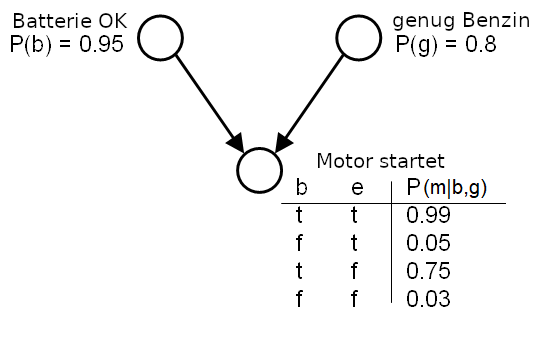
\includegraphics[width=0.6\textwidth]{bayes-netz-bsp.PNG}
	\caption{Bayes-Netz-Beispiel \cite{10}}
	\label{fig}
\end{figure}
\subsection{Problog}
\texttt{Problog} ist eine probabilistische Erweiterung von \texttt{Prolog} (PROgramming in LOGic), wobei \texttt{Prolog} eine logische Programmiersprache ist, die aus verschiedenen Klauseln $k_i$ und aus logischen Verknüpfungen ein Ergebnis berechnet. \texttt{Problog} erweitert jedes $k_i$ mit einer Wahrscheinlichkeit $p_i$, wodurch dies Wahrscheinlichkeiten ausgibt, mit welcher die $k_i$ eintreten, wohingegen \texttt{Prolog} nur ein Ergebnis nach logischen Berechnungen liefert und somit keine Angaben zu Wahrscheinlichkeiten unterstützt. \\  Ein probabilistischer Fakt lässt sich durch $p_i :: k_i$ definieren und weist einer Klausel die Wahrscheinlichkeit zu. Eine logische Verknüpfung $\land$ wird in \texttt{Problog} mit einem \enquote{,} dargestellt und eine Negation mit  \enquote{\textbackslash+}. Ein Beispiel für ein \texttt{Problog} Programm ist in \autoref{code:problogbeispiel} zu sehen.
\uzldeflanguageshorthand{Problog}{style=code,language=problog}
\begin{Pseudocode}[caption={\texttt{Problog} Programm-Beispiel}, label={code:problogbeispiel}, numbers=left]
0.1::erdbeben.
0.9::alarm_bei_erdbeben.
alarm :- erdbeben, alarm_bei_erdbeben.
\end{Pseudocode} 
Ein \texttt{Problog} Programm $T = {p_1 :: k_1, \dots, p_n :: k_n}$ gibt somit eine probabilistische Verteilung über die einzelnen Klauseln an und diese können anschließend zu einer beliebigen logischen Verknüpfung aus $K = {k_1 , \dots , k_n}$ verknüpft werden. In Beispiel 1 sieht man, dass der Fakt \textit{erdbeben} mit Wahrscheinlichkeit $ P(erdbeben) = 0.1$ wahr ist und $0.9$ falsch ist. Andersherum ist für den Fakt alarm\_bei\_erdbeben  die Wahrscheinlichkeit $0.9$, dass der Alarm auslöst und die Gegenwahrscheinlichkeit $0.1$, dass dieser nicht auslöst. Die Aussagen aus Zeile 1 und 2 sind probabilistische Fakten.  In Beispiel 1 gilt somit $P(alarm) = P(erdbeben) * P(alarm_bei_erdbeben) = 0.9 * 0.1 = 0.09$ \cite{4}\cite{5}. \\ 
Noch ein Konstrukt, das von \texttt{Problog} geliefert wird, ist die \textit{annotated disjunction}, die es möglich macht Klauseln zu definieren, die mehr als nur zwei Werte annehmen können. Dafür werden alle möglichen Werte die eintreffen können als probabilistischen Fakt dargestellt, jedoch wird diesen ein Tupel $t = (v,c) $ übergeben, wobei $v$ eine festgelegte Variable ist und $c \in \mathbb{N}$ eine Konstante, die den zutreffenden Wert repräsentiert, und  mit einem logischen $\lor$ verknüpft, das in \texttt{Problog} mit einem \enquote{,} dargestellt wird. Ein Beispiel dafür ist in \autoref{code:annotateddisjunction} zu sehen, dass einen Alarm beschreibt, der die Werte $P(A_1) = 0.2$ (an), $P(A_2) = 0.7$ (aus) oder $P(A_3) = 0.1$ (defekt) annehmen kann \cite{5}.
\begin{Pseudocode}[caption={\texttt{Problog}-Beispiel \textit{annotated disjunction}}, label={code:annotateddisjunction}, numbers=left]
2/10::alarm(X, 1); 7/10::alarm(X, 2); 1/10::alarm(X, 3).
\end{Pseudocode}

\subsection{\texttt{ATKLOG}} \label{sub:atklog}
Angerona verwendet \texttt{ATKLOG}, um ein Angreifermodell zu modellieren. \texttt{ATKLOG} ist eine Sprache die auf \texttt{Problog} basiert und entworfen wurde, um das initiale Vorwissen eines Benutzers über den Datenbankzustand darzustellen. Das Vorwissen des Benutzers wird als Wahrscheinlichkeitsverteilung definiert. Außerdem verändert sich das Vorwissen eines Benutzers in \texttt{ATKLOG}, wenn dieser eine Anfrage stellt, da das Ergebnis dem Benutzer mehr Informationen über den aktuellen Datenbankzustand verrät. Beachtet wird auch, dass verweigerte Anfragen das Vorwissen des Benutzers auch beeinflussen \cite{guarnieri2017securing}. \\ 
Ein syntaktischer Unterschied von \texttt{ATKLOG} zu \texttt{Problog} ist, dass eine Negation mit \enquote{\textit{NOT}} dargestellt wird. Außerdem werden \textit{annotated disjunctions} anders dargestellt, weil \texttt{ATKLOG} nur Variablenzuweisung oder probabilistische Fakten erlaubt. \\ Umgewandelt wird eine \textit{annotated disjunction} $v_1::a_1, ..., v_n::a_n$ in ein \texttt{ATKLOG} konformes Schema, indem das \enquote{;} entfernt und für jeden Wert den die Variable annehmen kann, eine neue Klausel erstellt wird. Anschließend wird jede Klausel mit einer neuen Variable, die im Folgenden $sw_1, \dots sw_n$ genannt werden, konjugiert und die dazugehörige Wahrscheinlichkeit mit $v_i$ für $1 \leq i < n$ wird für jeder dieser neu erstellen Variable ein probabilistischer Fakt hinzugefügt. Jedes $p_i$ wird dabei neu berechnet mit $v_i = p_i \cdot (1 - \sum_{1\leq j<i}p_i)^{-1}$, wobei $p_1, \dots ,p_{n-1}, p_n$ die Wahrscheinlichkeiten für das eintreffen der Werte sind.
Außerdem muss für jeden möglichen eintreffenden Wert ein Variablenname zugeordnet werden, der als $name$ definiert wird und die Tupel, die durch die \textit{annotated disjunction} übergeben werden als $\overline{t}_1 , \dots , \overline{t}_n$. Der Ausdruck $v::sw(\_)$ ist eine Abkürzung dafür, dass ein probabilistischer Wert für $v::sw(\overline{t})$ für jedes Tupel $\overline{t}$ existiert. Ein Muster für die Vorgehensweise bei \textit{annotated disjunction} ist in \autoref{annotateddisj} zu sehen.
\begin{Pseudocode}[caption={Vorgehensweise bei \textit{annotated disjunction}}, label={annotateddisj}, numbers=left]
$name(\overline{t}_1)$ :- $sw_1(\overline{t}_1)$
$\dots$
$name(\overline{t}_n)$ :- NOT $sw_1(\overline{t}_1), \dots ,$ NOT $sw_{n−1}(\overline{t}_{n−1}), sw_n(\overline{t}_n)$
	
$v_1::sw_1(\_)$
$\dots$
$v_n::sw_n(\_)$
\end{Pseudocode} 

\subsection{Angerona}
Angerona ist ein DBIC-Mechanismus \cite{22} der Datenbanken gegen probabilistische Inferenzen absichert. Es existiert zur Zeit nur ein Prototyp von Angerona, der nur boolesche Anfragen unterstützt. Es wurde zwar eine Lösung für nicht-boolesche Anfragen im Paper vorgestellt, jedoch wurde diese nicht im Prototypen implementiert.
\begin{algorithm}[ht]
	\caption{Angerona Algorithmus}\label{alg-angerona}
	\begin{algorithmic}[1]
		\State \textbf{Input} Systemzustand $s=\langle db,U,P\rangle $, Historie $h$, Aktion $\langle u,q \rangle$, Systemkonfiguration $C$ und ein ATKLOG Modell $ATK$
		\State \textbf{Output} Die Sicherheitsentscheidung ob die Anfrage q zugelassen wird in $\{ \top, \bot \}$
		\For{$\langle u, \psi, l \rangle \in$ secrets(P, u)}
		\If{$secure(C, ATK, h,\langle u,\psi,l \rangle$)}
		\If{ $pox(C, ATK, h, \langle u,q \rangle$)} \State 
		$h'\gets h \cdot \langle \langle u,q\rangle , \top , \top \rangle$
		\If{$ \neg secure(C, ATK, h',\langle u,\psi,l \rangle$}
		\State \textbf{return} $\bot$
		\EndIf
		\EndIf
		\If{ $pox(C, ATK, h, \langle u, \neg q \rangle$)} \State 
		$h'\gets h \cdot \langle \langle u, q\rangle , \top , \bot \rangle$
		\If{$ \neg secure(C, ATK, h',\langle u,\psi,l \rangle$}
		\State \textbf{return} $\bot$
		\EndIf
		\EndIf
		\EndIf
		\EndFor
		\State \textbf{return} $\top$
		\State
		\Function{secure}{$\langle D,\Gamma \rangle$, ATK, h, $\langle u, \psi , l \rangle$}
		\State $p\gets ATK(u)$
		\For{$\phi \in knowledge(h,u)$} 
		\State $p\gets p \cup PL(\phi) \cup \{evidence(head(\phi),true)\}$ 
		\EndFor
		\State $p\gets p\cup PL(\psi)$
		\State \textbf{return} $\lsem p \rsem_D   (head(\psi)) < l $
		\EndFunction
		\State
		\Function{$pox$}{$\langle D,\Gamma \rangle, ATK,h,\langle u,\psi \rangle $}
		\State $p\gets ATK(u)$
		\For{$\phi \in knowledge(h,u)$} 
		\State $p\gets p \cup PL(\phi) \cup \{evidence(head(\phi),true)\}$ 
		\EndFor
		\State $p\gets p\cup PL(\psi)$
		\State \textbf{return} $\lsem p \rsem_D   (head(\psi)) > 0 $
		\EndFunction
	\end{algorithmic}
\end{algorithm}
Der Angerona Algorithmus aus \autoref{alg-angerona} erhält folgende Eingaben:
\begin{itemize}
	\item Den Systemzustand $s=\langle db,U,P\rangle $ der den aktuellen Systemzustand beschreibt, wobei $db$ der aktuelle Datenbankzustand ist, $U$ die Menge der Benutzer und $P$ die Sicherheitsregeln enthält.
	\item Die Historie H, die aus einer Sequenz $h=\langle \langle u,q \rangle ,d,a \rangle$ besteht, die für jeden Benutzer alle bereits getätigten Anfragen speichert. Jeder Eintrag in der Historie speichert den Benutzer $u$, die Anfrage $q$, die Entscheidung $d \in \{\top, \bot \}$, ob die Anfrage genehmigt wurde und die Antwort aus dem Datenbanksystem $a \in \{\top, \bot , \dag \} $, wobei $\dag$ die Antwort ist, wenn die Anfrage nicht genehmigt wurde.
	\item Die Aktion $\langle u,q \rangle$ die eine Anfragen $q$ einem Benutzer $u$ zuordnet, die  an Angerona gestellt wird.
	\item Die Systemkonfiguration $C$, die aus $\langle D,\Gamma \rangle$ besteht, wobei $D$  das Datenbankschema darstellt und $\Gamma$ die Integritätsbedingungen. 
	\item  Das $ATKLOG$ Modell $ATK$, dass das Angreifermodell für jeden Benutzer $u$ über das aktuelle Datenbankschema darstellt.
\end{itemize}
Angerona verwendet außerdem noch einige Funktionen innerhalb der \texttt{secure} und \texttt{pox} Funktionen. Diese sind zum einen die Funktion \texttt{knowledge}, die aus der Historie $h$ alle extrahiert, die zum Benutzer $u$ gehören.\\
Zum anderen die Funktion \texttt{evidence}, die aus \texttt{Problog} stammt und verwendet wird, um Informationen als wahr oder falsch anzunehmen, was dadurch die Wahrscheinlichkeitswerte für andere probabilistische Abhängigkeitsregeln verändert.\\ 
Die Funktion \texttt{PL}, die  eine Anfrage in logische Programmierregeln umwandelt und somit für \texttt{Problog} lesbar macht \cite{guarnieri2017securing}.  \\ \\
Der Algorthmus prüft dabei für die Anfrage $q$, welche der Benutzer $u$ gestellt hat aus der Aktion $\langle u,q \rangle$, ob diese eine Sicherheitsregel aus $secrets(P,u)$ verletzt und gibt $\top$ zurück, wenn die Anfrage genehmigt oder $\bot$ wenn diese verweigert werden soll. \\ 
Dafür wird über alle  $secrets(P,u) = \{ \langle u,\phi,l \rangle \mid \langle u,\phi,l \rangle \in P \land u \in U\}$ iteriert, wobei $\phi$ die Anfrage und $l$ den Schwellwert definiert, bei der die Anfrage verweigert werden soll. In jeder Iteration für jede Sicherheitsregel wird zuerst geprüft, ob die Sicherheitsregel bereits verletzt wurde, indem zuerst die Funktion \texttt{secure} ausgeführt wird. \\ 
Die Funktion \texttt{secure} erweitert dafür das aktuelle Angreifermodell $ATK$, indem alle bereits getätigten Anfragen aus der Historie $h$ von dem Benutzer $u$ hinzufügt werden und als \texttt{evidence} markiert werden. Anschließend wird mit der Funktion \texttt{PL} die Anfrage aus der Sicherheitsregel noch in \texttt{Problog} definiert und dem Angreifermodell hinzugefügt. Der Ausdruck $\lsem p \rsem_D (head(\psi)$ prüft dabei für alle Datenbankzustände, in welcher die Anfrage $\psi$ erfüllt ist und berechnet die Wahrscheinlichkeit durch (Menge der Datenbankzustände in den $\psi$ erfüllt ist)/(Menge aller Datenbankzustände). Wenn diese Wahrscheinlichkeit kleiner dem Schwellwert $l$ ist, dann gilt die Sicherheitsregel als nicht verletzt und es wird ein $\top$ ausgegeben. \\ 
Anschließend wird sichergestellt, dass die Sicherheitsentscheidung selbst keine Informationen verrät, indem das Vorwissen vom Benutzer $u$ unter dem Schwellwert $l$ liegen muss, für die Fälle, dass $q$ genehmigt und das $q$ verweigert wurde. Dafür wird mit der Funktion $pox$ geprüft , ob ein Datenbankzustand für das Datenbankmodell existiert in dem $q$ erfüllt ist. Dabei geht die Funktion $pox$ die selben Schritte wie die Funktion $secure$ durch, vergleicht am Ende jedoch die Wahrscheinlichkeit der erfüllenden Datenbankzustände nicht mit dem Schwellwert sondern prüft nur, ob diese größer 0 ist. Wenn $pox$ ein $\top$ zurückgibt und somit ein Datenbankzustand existiert, indem $q$ erfüllt ist, wird eine neue Historie $h'$ erstellt, die um die Anfrage $q$ erweitert ist. Anschließend wird die \texttt{secure} Funktion mit der neuen Historie $h'$ ausgeführt und geprüft, ob die Sicherheitsregel verletzt wird, wenn die Anfrage $q$ genehmigt wurde. Damit wird verhindert, dass eine genehmigte Anfrage eine andere Sicherheitsregel verletzen würde. Wenn die erweiterte Historie $h'$ die Sicherheitsregel verletzt, dann verweigert Angerona die Anfrage $q$ gibt somit ein $\bot$ als Output. \\ 
Danach werden die selben Schritte für die Anfrage $\neg q$ durchgeführt, die beschreibt, dass die Anfrage nicht genehmigt wurde. Dafür wird wieder mit der Funktion $pox$ geprüft, ob ein Datenbankzustand existiert, indem $ \neg q$ gilt. Wenn dies der Fall ist, dann wird die Historie $h'$ um die Anfrage $\neg q$ erweitert und es wird geprüft, ob durch die Verweigerung der Anfrage $q$ die Sicherheitsregel verletzt wird. Wenn dies nicht der Fall ist, wird von Angerona ein $\top$ ausgegeben, ansonsten ein $\bot$. \\ \\ 
\section{Praktisches Setup} \label{2.2}
Der Prototyp von Angerona kann auf der Webseite von Marco Guarnieri \cite{6} heruntergeladen werden. Angerona lässt sich in zwei verschiedenen Modis starten :
\begin{enumerate}
	\item \textbf{Experiment}: Hiermit können vorgefertigte Beispiele aus dem Paper \enquote{Securing Databases from Probabilistic Inference} \cite{guarnieri2017securing} reproduziert werden. Dadurch werden keine größeren Initialisierungsschritte benötigt und das Programm übernimmt die Generierung vom Angreifermodell und die dazugehörige Datenbank. Anschließend werden zufällig generierte Anfragen an die Datenbank gestellt und von Angerona geprüft. Als Ergebnis vom Programm erhält man die Zeitmessung für die Ausführung der Anfrage, die Ausführungszeit von Angerona und die gesamte Zeit in einer CSV Datei.
	\item \textbf{Manual}: Erlaubt es mit Angerona eine Datenbank abzusichern und Anfragen über Angerona an diese zu stellen.
	In diesem Modus erwartet Angerona jeweils den Pfad zu den Dateien \texttt{beliefProgram.pbl}, \texttt{initStatements.txt} und \texttt{template.cpt} als Argument bei Programmstart.
\end{enumerate}
Im Folgenden wird ausschließlich der Manual Modus verwendet. Das Problem jedoch ist, dass es noch keine Dokumentation zu Angerona gibt und nur eine mitgelieferte \texttt{README} in der beschrieben wird, wie sich Angerona starten lässt. Jedoch wird nicht beschrieben wie die drei mitgelieferten Dateien definiert werden können. Deshalb wurde anhand von Beispielen im Code und Inhalten aus dem Paper hergeleitet, wie die Dateien für den Input erstellt und wie Anfragen über Angerona gestellt werden können.
\subsection{Angreifermodell} \label{2.2.1}
Das Angreifermodell wird in der Datei \texttt{beliefProgram.pbl} beschrieben. Hier wird das Vorwissen des Angreifers mithilfe von \texttt{ATKLOG} beschrieben, dass auf \texttt{Problog} basiert. Dabei übernimmt das Angreifermodell die Aufgabe, das Vorwissen jedes Benutzers für jeden Patienten in der Datenbank zu modellieren. \\ 
Hierfür wird zuerst ein Bayes-Netz für die abzusichernden sensiblen Daten und deren Abhängigkeiten mit den probabilistischen Wahrscheinlichkeiten modelliert. Anschließend wird das Bayes-Netz in zwei Schritten in das Angreifermodell überführt. Im ersten Schritt wird das Bayes-Netz in ein \texttt{Problog}-Programm überführt. Das \texttt{Problog}-Programm enthält noch syntaktischen Zucker, wie zum Beispiel die \emph{annotated disjunctions}, der von Angerona nicht unterstützt wird. Entsprechend wird wie in \cref{sub:atklog} beschrieben das \texttt{Problog}-Programm  in ein \texttt{ATKLOG}-konformes Schema überführt. Diese Schritte müssen manuell durchgeführt werden. \\   
Dann werden alle Knoten $\{v_0, \dots ,v_n\} \in V$ aus dem Bayes-Netz in das Angreifermodell übertragen, die \textbf{keine Abhängigkeit} besitzen. Diese sind definiert als $\{np_i \in V \mid Parent(np_i) = \emptyset\}$, wobei das Attribut \textit{name} dem vorher definierten Namen des Knotens entspricht. Dafür werden zuerst die Knoten einer Variable zugeordnet und anschließend die Wahrscheinlichkeiten für die Variable als probabilistischen Fakt für jeden Patienten $p \in \mathbb{N}$ in das Angreifermodell hinzugefügt, wie im \autoref{code:beliefprogramOhneInference} zu sehen ist. 
\newpage
\begin{Pseudocode} [caption={\texttt{beliefProgram.pbl} für Knoten ohne Abhängigkeiten}, label={code:beliefprogramOhneInference}, numbers=left]
$np_0.name(X) :- p\_np_0.name(X).$ 
$np_1.name(X) :- p\_np_1.name(X).$ 
$\dots$
$np_n.name(X) :- p\_np_n.name(X).$

$P(np_0) ::  p\_np_0.name(p_0).$ 
$P(np_1) ::  p\_np_1.name(p_0).$ 
$\dots$
$P(np_n) ::  p\_np_n.name(p_0).$ 
$P(np_0) ::  p\_np_n.name(p_1).$ 
$\dots$
$P(np_0) ::  p\_np_0.name(p_n).$ 
$P(np_1) ::  p\_np_1.name(p_n).$ 
$\dots$
$P(np_n) ::  p\_np_n.name(p_n).$ 
\end{Pseudocode}
Für die Knoten \textbf{mit Abhängigkeiten}, also für alle Knoten $V$ für die gilt $H=\{v \in V \mid \lvert Parent(v) \rvert \geq 1 \}$ werden die Klauseln für jede mögliche Welt von den Abhängigkeiten $a_0, ... a_n$ eingefügt und verknüpft mit einer Konjunktion, die in \texttt{ATKLOG} mit einem $","$ dargestellt wird. Anschließend wird jeder Ausdruck mit einer selbst definierten Variable versehen und mit diesem konjugiert, die am Ende durch einen probabilistischen Fakt die dazugehörige Wahrscheinlichkeit für diese Welt zuordnet. Ein Beispiel für ein Bayes-Netz mit zwei Abhängigkeiten ist in \autoref{example-bayes-net-with-abh}  und die dazugehörige \texttt{beliefProgram.pbl} in \autoref{code:beliefprogramMitInference} zu sehen.
\begin{figure}[ht]
	\caption{Bayes-Netz mit 2 Abhängigkeiten}
	\label{example-bayes-net-with-abh}
	\centering
	\begin{tikzpicture}[
		node distance=1cm and 0cm,
		mynode/.style={draw,ellipse,text width=2cm,align=center}
		]
		\node[mynode] (wp) {$h_0.name$};
		\node[mynode,above right=of wp] (npeins) {$a_1.name$};
		\node[mynode,above left=of wp] (npnull) {$a_0.name$};
		\path 
		(npnull) edge[-latex] (wp)
		(npeins) edge[-latex] (wp);
		\node[above=0.2cm of npnull]
		{
			\begin{tabular}{|c|}
				\hline
				$a_0.name$ \\
				$P(A)$ \\
				\hline
				$P(a_0)$ \\
				\hline
			\end{tabular}
		};
		\node[above=0.2cm of npeins]
		{
			\begin{tabular}{|c|}
				\hline
				$a_1.name$ \\
				$P(B)$ \\
				\hline
				$P(a_1)$ \\
				\hline
			\end{tabular}
		};
		\node[below=0.2cm of wp]
		{
			\begin{tabular}{|c|c|c|}
				\hline
				\multicolumn{3}{|c|}{$h_0.name$} \\
				\hline
				A & B &$P(C|A,B)$ \\
				\hline
				T&T& $P(h_0)$ \\
				T&F &$P(h_1)$ \\
				F&T &$P(h_2)$ \\
				F&F &$P(h_3)$ \\
				\hline
			\end{tabular}
		};
	\end{tikzpicture}
\end{figure}
\\
\begin{Pseudocode}[caption={\texttt{beliefProgram.pbl} für Knoten mit Abhängigkeiten}, label={code:beliefprogramMitInference}, numbers=left]
$H(X)$ :- $a_0.name(X)$ , $a_1.name(X)$, $variable11(X).$
$H(X)$ :- $a_0.name(X)$ , $NOT a_1.name(X)$, $variable10(X).$
$H(X)$ :- NOT $a_0.name(X)$ , $a_1.name(X)$, $variable01(X).$
$H(X)$ :- NOT $a_0.name(X)$ , $NOT a_1.name(X)$, $variable00(X).$

$P(h_0) :: variable11(p_0)$
$P(h_1) :: variable10(p_0)$
$P(h_2) :: variable01(p_0)$
$P(h_n) :: variable00(p_0)$
$\dots$
$P(h_0) :: variable11(p_n)$
$P(h_1) :: variable10(p_n)$
$P(h_2) :: variable01(p_n)$
$P(h_n) :: variable00(p_n)$
\end{Pseudocode} 
Eine \textbf{mehrwertige Variable} kann anstatt zwei Wahrheitswerten \texttt{true} und \texttt{false} auch mehr Werte annehmen.
Um diese im Angreifermodell auszudrücken, wird die mehrwertige Variable in eine \textit{annotated disjunction} eingeteilt. Zum Beispiel das Alter einer Person kann mehrere Werte annehmen. Im Folgenden Beispiel wird das Alter einer Person in jung, mittel(alt) und alt eingeteilt. Dabei sind die Wahrscheinlichkeiten dafür, dass eine Person jung ist $40\%$, mittel $25\%$ und alt $35\%$. Dann würde im \texttt{beliefProgram.pbl} die Klauseln wie in \autoref{code:mehrwertigeVariable} zu sehen ist, angeordnet werden und die Wahrscheinlichkeiten $p_i$ jeweils berechnet werden durch : 
\begin{itemize}
	\item $0.4 \cdot (1- 0)^{-1} = 0.4 $
	\item  $0.25 \cdot (1 - 0.4)^{-1} = 0.4166 = 5/12 $
	\item $ 0.35 \cdot (1 - 0.35 - 0.4)^{-1} = 1 $
\end{itemize}
\begin{Pseudocode}[caption={Beispiel für mehrwertige Variablen}, label={code:mehrwertigeVariable}]
alter(X,1) :- p_jung(X).
alter(X,2) :- NOT p_jung(X), p_mittel(X).
alter(X,3) :- NOT p_jung(X) , NOT p_mittel(X) , p_alt(X).

4/10 :: p_jung(id).
5/12 :: p_mittel(id).
1/1 :: p_alt(id).
\end{Pseudocode} 


\subsection{Initialisierung und Sicherheitsregeln}
Die \texttt{initStatements.txt} definiert das Datenbankschema und füllt die Datenbank mit Daten. Außerdem werden hier die Sicherheitsregeln definiert, die den Schwellwert festlegen, bei dem ein Benutzer auf die Daten der Datenbank zugreifen darf.. \\ \\  
Die \texttt{initStatements.txt} wird in vier Schritte initialisiert:
\begin{enumerate}
	\item Die \textbf{Tabellen } werden mit dem Kommando \textit{AS admin : CREATE TABLE tablename(attribute)} initialisiert. 
	\item  Die \textbf{Benutzer} werden mit dem Kommando \textit{AS admin : ADD USER benutzer} initialisiert. 
	\item Die \textbf{Sicherheitsregeln}  werden mit dem Kommando \textit{AS admin : SECRET anfrage('id') FOR benutzer THRESHOLD schwellwert} initalisiert.
	\item Das \textbf{Füllen} der Datenbank wird mit dem Kommando \textit{AS admin : INSERT IN tabelle ['id']} erledigt.
\end{enumerate} 
\subsection{Template}
Die \texttt{template.cpt} ist die Vorlage für Angerona. In dieser werden die Tabellen aus den \texttt{initStatements.txt} und die definierten Fakten aus dem \texttt{beliefProgram.pbl} initialisiert.

\section{Beispiel} \label{chap:Beispiel}
In diesem Beispiel wird  eine medizinische Datenbank eines Krankenhauses betrachtet, die das Rauchverhalten und die Elternbeziehung von Patienten speichert und ob diese Krebs haben. Die Datenbank hat dabei die Tabellen \textit{Patienten, Raucher, Krebs, MutterHatKrebs } und \textit{VaterHatKrebs}. In der medizinischen Datenbank sind die Patienten Alice mit der \textit{id} 1, Bob mit der \textit{id} 2 und Carl mit der \textit{id} 3 definiert, wobei Alice und Bob die Eltern von Carl sind. Alice raucht nicht, aber Bob und Carl rauchen. Alice und Bob haben Krebs und Carl hat keinen Krebs. Der Benutzer für das System ist Mallory mit dem Benutzernamen \textit{mallory}. Außerdem wird vom folgendem probabilistischen Modell ausgegangen: 
\begin{enumerate}
\item Jeder Patient entwickelt mit einer Wahrscheinlichkeit von 5\% Krebs
\item Für jeden Elternteil, der Krebs hat, steigt die Wahrscheinlichkeit für das Kind Krebs zu bekommen, um 15\%
\item Wenn ein Patient raucht, steigt die Wahrscheinlichkeit, dass dieser Krebs bekommt, um  25\%
\end{enumerate}
Zu Beginn  wird das probabilistische Modell in ein Bayes-Netz übertragen. Dabei wird davon ausgegangen, dass die Wahrscheinlichkeit dafür, dass ein Patient raucht 25\% und dass jeweils ein Elternteil Krebs hat 10\% entspricht \cite{11}. Ein Patient ist in diesem Fall zu 100\% ein Patient, da eine medizinische Datenbank betrachtet wird \cite{guarnieri2017securing}. Dadurch ergibt sich das Bayes-Netz aus \autoref{tikz-1}.
\begin{figure}[htbp]
	\caption{Bayes-Netz}
	\label{tikz-1}
	\centering
	\begin{tikzpicture}[
		node distance=1cm and 0cm,
		mynode/.style={draw,ellipse,text width=2cm,align=center}
		]
		\node[mynode] (patient) {Patienten};
		\node[mynode,right=of patient] (smokes) {Raucher};
		\node[mynode,right=of smokes] (mother) {MutterHatKrebs};
		\node[mynode,right=of mother] (dad) {VaterHatKrebs};
		\node[mynode,below right=of smokes] (cancer) {Krebs};
		\path 
		(patient) edge[-latex] (cancer)
		(mother) edge[-latex] (cancer)
		(smokes) edge[-latex] (cancer) 
		(dad) edge[-latex] (cancer);
		\node[above=0.5cm of patient]
		{
			\begin{tabular}{|c|}
				\hline
				Patienten \\
				$P(P)$ \\
				\hline
				$1.00$\\
				\hline
			\end{tabular}
		};
		\node[above=0.5cm of smokes]
		{
			\begin{tabular}{|c|}
				\hline
				Raucher \\
				$P(R)$ \\
				\hline
				$0.25$ \\
				\hline
			\end{tabular}
		};
		\node[above=0.5cm of mother]
		{
			\begin{tabular}{|c|}
				\hline
				Mutter hat Krebs \\
				$P(M)$ \\
				\hline
				$0.1$ \\
				\hline
			\end{tabular}
		};
		\node[above=0.5cm of dad]
		{
			\begin{tabular}{|c|}
				\hline
				Vater hat Krebs \\
				$P(V)$ \\
				\hline
				$0.1$ \\
				\hline
			\end{tabular}
		};
		\node[below=0.5cm of cancer]
		{
			\begin{tabular}{|c|c|c|c|c|}
				\hline
				\multicolumn{5}{|c|}{Krebs} \\
				\hline
				P &R & M &V &$P(K|P,R,M,V)$ \\
				\hline
				T&T&T&T& $0.6$ \\
				T&T&T&F& $0.45$\\
				T&T&F&T& $0.45$\\
				T&T&F&F& $0.3$\\
				T&F&T&T& $0.35$\\
				T&F&T&F& $0.2$\\
				T&F&F&T& $0.2$\\
				T&F&F&F& $0.05$\\
				\hline
			\end{tabular}
		};
	\end{tikzpicture}
\end{figure} 
Die Fälle mit $P$=\textit{false} sind bewusst nicht in der Tabelle für Krebs gelistet, da diese Fälle nicht eintreffen können. Die Wahrscheinlichkeiten dafür, dass ein Patient Krebs hat wird berechnet, indem die oben genannten Wahrscheinlichkeiten aufsummiert werden, wenn dieser Fakt auf den Patienten zutrifft. Zum Beispiel der Wert in der ersten Tabellenzeile ergibt sich aus $0.05 + 0.15 + 0.15 +0.25 = 0.6$.
Mithilfe des Bayes-Netzes wird das Angreifermodell definiert, indem zuerst jeder Knoten der keine Abhängigkeiten besitzt, definiert wird, wie in Kapitel \cref{2.2} beschrieben. Im Beispiel sind das die Knoten Patient, Raucher, MutterHatKrebs und VaterHatKrebs. Dadurch ergibt sich für die \texttt{beliefProgram.pbl} der Code aus \autoref{lst-3}
\begin{Pseudocode}[caption={Beispiel für Knoten ohne Abhängigkeiten }, label={lst-3}, numbers=left]
patient(X) :- p_patient(X).
raucher(X) :- p_raucher(X).
mutterhatkrebs(X) :- p_mutterhatkrebs(X).
vaterhatkrebs(X) :- p_vaterhatkrebs(X).
	
1/1 :: p_patient(1).
25/100 :: p_raucher(1).
1/10 :: p_mutterhatkrebs(1).
1/10 :: p_vaterhatkrebs(1).
1/1 :: p_patient(2).
25/100 :: p_raucher(2).
1/10 :: p_mutterhatkrebs(2).
1/10 :: p_vaterhatkrebs(2).
1/1 :: p_patient(3).
25/100 :: p_raucher(3).
1/10 :: p_mutterhatkrebs(3).
1/10 :: p_vaterhatkrebs(3).
\end{Pseudocode}
Anschließend können die Knoten mit Abhängigkeiten definiert werden. Im Beispiel ist das nur der Knoten Krebs. Für den Knoten Krebs wird dafür für jede mögliche Welt in Abhängigkeiten von den Elternknoten eine Klausel initialisiert und mit einer selbst definiert Variable versehen, die im Folgenden die Form $v0000, v0001, \dots , v1111$ hat. Damit wird das \texttt{beliefProgral.pbl} erweitert um den Code aus \autoref{lst-abhangig} 
\begin{Pseudocode}[caption={Beispiel für Knoten mit Abhängigkeiten }, label={lst-abhangig}, numbers=left]
krebs(X) :- patient(X), raucher(X), mutterhatkrebs(X), vaterhatkrebs(X), v1111(X).
krebs(X) :- patient(X), raucher(X), mutterhatkrebs(X), NOT vaterhatkrebs(X), v1110(X).
krebs(X) :- patient(X), raucher(X), NOT mutterhatkrebs(X), vaterhatkrebs(X), v1101(X).
krebs(X) :- patient(X), raucher(X), NOT mutterhatkrebs(X), NOT vaterhatkrebs(X), v1100(X).
krebs(X) :- patient(X), NOT raucher(X), mutterhatkrebs(X), vaterhatkrebs(X), v1011(X).
krebs(X) :- patient(X), NOT raucher(X), mutterhatkrebs(X), NOT vaterhatkrebs(X), v1010(X).
krebs(X) :- patient(X), NOT raucher(X), NOT mutterhatkrebs(X), vaterhatkrebs(X), v1001(X).
krebs(X) :- patient(X), NOT raucher(X), NOT mutterhatkrebs(X), NOT vaterhatkrebs(X), v1000(X).

6/10 :: v1111(1).
45/100 :: v1110(1).
45/100 :: v1101(1).
3/10 :: v1100(1).
35/100 :: v1011(1).
2/10 :: v1010(1).
2/10 :: v1001(1).
5/100 :: v1000(1).
6/10 :: v1111(2).
45/100 :: v1110(2).
45/100 :: v1101(2).
3/10 :: v1100(2).
35/100 :: v1011(2).
2/10 :: v1010(2).
2/10 :: v1001(2).
5/100 :: v1000(2).
6/10 :: v1111(3).
45/100 :: v1110(3).
45/100 :: v1101(3).
3/10 :: v1100(3).
35/100 :: v1011(3).
2/10 :: v1010(3).
2/10 :: v1001(3).
5/100 :: v1000(3).
\end{Pseudocode}
Damit wäre das Angreifermodell mit dem \textit{beliefProgram.pbl} vollständig initialisiert.\\ \\
Die \texttt{initStatements.txt} werden nach den vorher angegeben vier Schritten initialisiert.
\begin{enumerate}
	\item  Für jeden Knoten aus dem Bayes-Netz wird eine \textbf{Tabelle} angelegt: 
\begin{Pseudocode}
AS admin : CREATE TABLE patient(id)
AS admin : CREATE TABLE raucher(id)
AS admin : CREATE TABLE mutterhatkrebs(id)
AS admin : CREATE TABLE vaterhatkrebs(id)
AS admin : CREATE TABLE krebs(id)
\end{Pseudocode}
\item Der \textbf{Benutzer} Mallory wird folgendermaßen angelegt:
\begin{Pseudocode}
AS admin : ADD USER mallory
\end{Pseudocode}
\item Die \textbf{Sicherheitsregeln} können beliebig gewählt werden. Im Folgenden darf Mallory auf die Daten nur zugreifen, wenn sie mit einer Wahrscheinlichkeit von unter 50\% weiß, dass ein beliebiger Patient Krebs hat.
\begin{Pseudocode}
AS admin : SECRET krebs('1') FOR mallory THRESHOLD 1/2
AS admin : SECRET krebs('2') FOR mallory THRESHOLD 1/2
AS admin : SECRET krebs('3') FOR mallory THRESHOLD 1/2
\end{Pseudocode}
\item \textbf{Gefüllt} wird die Datenbank mit den oben gegeben Werten dann folgendermaßen:
\begin{Pseudocode}
AS admin : INSERT IN patient['1']
AS admin : INSERT IN patient['2']
AS admin : INSERT IN patient['3']
AS admin : INSERT IN raucher['2']
AS admin : INSERT IN raucher['3']
AS admin : INSERT IN mutterhatkrebs['1']
AS admin : INSERT IN vaterhatkrebs['1']
AS admin : INSERT IN krebs['1']
AS admin : INSERT IN krebs['2']
\end{Pseudocode}
\end{enumerate}
In der  \texttt{tempalte.cpt} werden alle verwendeten Variablen aus der \texttt{beliefProgram.pbl} und \texttt{initStatements.txt} wie in \autoref{code:templatecpt} initalisiert.
\begin{Pseudocode}[caption={\texttt{tempalte.cpt} vom Beispiel} , label = {code:templatecpt} , numbers=left]
patient: []
raucher: []
mutterhatkrebs: []
vaterhatkrebs: []
p_patient: []
p_raucher: []
p_mutterhatkrebs: []
p_vaterhatkrebs: []
krebs: []
v1111: []
v1110: []
v1101: []
v1100: []
v1011: []
v1010: []
v1001: []
v1000: []
\end{Pseudocode}
Nun wird Angerona anhand der \texttt{prototype.jar} mit folgendem Befehl ausgeführt:
\begin{lstlisting}[language=bash]
java -jar prototype.jar angeronaManual 1 pfad/nach/beliefProgram.pbl pfad/nach/initStatements.txt pfad/nach/template.cpt
\end{lstlisting}
Anschließend können Anfragen mit Angerona gestellt werden mit dem Befehl \texttt{AS [user] : [tabelle]('[id]')}. Ein Beispiel für eine Anfrage von Mallory, ob Alice Krebs hat, ist in \autoref{code:anfragevonm} zu sehen.
\begin{Pseudocode}[caption={Angerona: Anfrage von Mallory ob Alice Krebs hat } , label = {code:anfragevonm} , numbers=left]
Write a command. Write 'Stop' to conclude.
AS mallory:krebs('1')
ACCESS CONTROL RESULT
Acc.Ctrl.: false Cause: mallory : krebs ('1') is not authorized
\end{Pseudocode}

\chapter{Medizinische Datenbanken und Angreifermodellierung}\label{chap:Modellierung}
In diesem Kapitel wird der Prototyp von Angerona auf drei verschiedene medizinische Datenbanken angewendet. Betrachtet werden die Datenbanken MIMIC-III, eICU und der synthetische Patientengenerator Synthea.
\section{MIMIC-III}
MIMIC-III (Medical Information Mart for Intensive Care) III ist eine für Forschungszwecke frei zugängliche Datenbank, die pseudonymisierte medizinische Daten und dazugehörige klinische Daten, die in Intensivstationen in einem Spezialkrankenhaus eingewiesen wurden, speichert. Die Daten stammen dabei aus dem \textit{Beth Israel Deaconess Medical Center} in Boston, Massachusetts und wurden in dem Zeitraum vom Juni 2001 bis Oktober 2012 erfasst. Die Datenbank enthält 58976 Krankenhauseinweisungen für 38645 Erwachsene und 7875 Neugeborene. Gespeichert werden Daten wie Vitalparameter, Medikamente, Labormessungen, Beobachtungen, Notizen vom Personal, Flüssigkeitsbilanzen, Verfahrenscodes, Diagnosecodes, Aufenthaltsdauer, Überlebensdaten und mehr \cite{12}.  \\ \\ 
Im Folgenden wird für jeden Patienten in der MIMIC-III-Datenbank die Information, dass dieser Krebs hat, abgesichert. Die Wahrscheinlichkeitswerte des Vorwissens vom Angreifermodell wird aus der MIMIC-III-Datenbank ausgelesen, indem zum Beispiel die Wahrscheinlichkeit für das Vorwissen, dass eine Person Krebs hat, berechnet wird durch $
P(krebs) =  \frac{\text{Anzahl der Patienten die Krebs haben}}{\text{Gesamtanzahl der Patienten}}$. \\ 
Risikofaktoren und somit Abhängigkeiten für Krebs sind in dem Fall Alter, Geschlecht und Rauchverhalten des Patienten \cite{13,14}. Um diese Daten aus der MIMIC-III-Datenbank zu erhalten werden die folgenden Tabellen benötigt : 
\begin{enumerate}
	\item Die Tabelle \textit{ADMISSIONS} enthält Informationen über die Einweisung ins Krankenhaus. Dabei ist jeder Krankenhausaufenthalt einer eindeutigen \textit{HADM\_ID} zugeordnet. Die Tabelle enthält Informationen zu demographischen Daten, Ein- und Ausweisungszeiten und erste Einweisungsinformationen.
	\item Die Tabelle \textit{PATIENTS} enthält Informationen über jeden Patienten. Dabei ist jeder Patient einer eindeutigen \textit{SUBJECT\_ID} zugeordnet und kann mehrere \textit{HADM\_ID} zugeordnet werden, weil ein Patient mehrmals ins Krankenhaus eingewiesen werden kann. Die Tabelle enthält Informationen über das Geschlecht, das Geburtsdatum und falls vorhanden das Todesdatum.
	\item Die Tabelle \textit{DIAGNOSES\_ICD} enthält pro \textit{HADM\_ID} und \textit{SUBJECT\_ID} die dazugehörige Diagnose als \texttt{icd9-code}(International Classification of Diseases). \texttt{Icd9-codes} sind standardisierte Codes, die verwendet  werden um Krankheiten , Verletzungen oder sonstige Diagnosen International einheitlich zu speichern \cite{15}.
	\item Die Tabelle \textit{NOTEEVENTS} enthält alle Notizen zu den Patienten, die vom Krankenhauspersonal dokumentiert sind.
\end{enumerate} 
Im Folgenden wird die Angreifermodellierung für die MIMIC-III-Datenbank anhand der Krankenhauseinweisungen betrachtet. Das bedeutet, dass die \textit{HADM\_ID} für die Zuordnung der Patienten genutzt wird, um diese nach Angerona zu übertragen. Daher kann es auch vorkommen, dass Patienten mehrmals auftauchen, wenn diese mehrmals eingewiesen wurden.\\ 
Das Alter wurde in die Intervalle $[0,40], (40,60]$ und $(60,\infty)$ eingeteilt, da diese als Altersgrenze definiert sind, in denen die Risiken für Krebs sich unterscheidet. Außerdem ist mit einem höherem Alter ein erhöhtes Krebsrisiko verbunden \cite{13}. Krankenhauseinweisungen für Patienten mit einem Alter im Intervall $[0,40]$ existieren 13265, für $(40,60]$ 14382 und $(60,\infty)$ 31329. Dies lässt sich berechnen, indem die Differenz zwischen dem Geburtsdatum aus der Tabelle \textit{PATIENTS} und dem Einweisungsdatum aus der Tabelle \textit{ADMISSIONS} berechnet wird.\\
Das Geschlecht jedes Patienten kann aus der Tabelle \textit{PATIENTS} unter dem Attribut \textit{gender} ausgelesen werden und es gibt 32950 Männer und 26026 Frauen, wobei Männer eine höhere Wahrscheinlichkeit haben Krebs zu bekommen als Frauen. \\
Das Rauchverhalten wurde aus der Tabelle \textit{NOTEEVENTS} ausgelesen, indem nach den Schlagwörtern \enquote{smoke} und \enquote{cigarette} gesucht wurde. Somit erhält man 25237 Raucher, wobei Raucher ein erhöhtes Risiko haben Krebs zu bekommen. \\
Um die Krankenhausaufenthalte zu erhalten, für die Patienten bei den  Krebs diagnostiziert wurde, werden die \texttt{icd9-codes} für Krebs \cite{16} mit den aus der \textit{DIAGNOSES\_ICD} verglichen und bei Gleichheit hinzugefügt. Dafür wurde ein Skript geschrieben, dass alle \texttt{icd9-codes} aus einer Liste, in der \texttt{icd9-codes} für Krebs notiert sind, extrahiert und in  das \texttt{icd9-code} Format von der MIMIC-III-Datenbank umwandelt und anschließend diese in eine extra angefertigte Tabelle kopiert. Somit kann man diese Tabellen direkt miteinander vergleichen und erhält 13658 Krebspatienten. \\ 
Diese Informationen werden mit einem Bayes-Netz grafisch dargestellt, dass in Abbildung \ref{mimic-bayes-net} zu sehen ist.\\
\begin{figure}[ht]
	\caption{MIMIC-III Bayes-netz}
	\label{mimic-bayes-net}
	\begin{tikzpicture}[
		node distance=1cm and 1.5cm,
		mynode/.style={draw,ellipse,text width=2cm,align=center}
		]
		\node[mynode] (age) {Age};
		\node[mynode,below right=of age] (cancer) {Cancer};
		\node[mynode,above right=of cancer] (smoke) {Smokes};
		\node[mynode,above = of cancer] (male) {Male};
		\path [-latex]
		(age) edge (cancer) 
		(male) edge(cancer) 
		(smoke) edge  (cancer);
		\node[above=0.4cm of age]
		{
			\begin{tabular}{|c|c|c|}
				\hline
				\multicolumn{3}{|c|}{Age} \\
				$P(A=[0,40])$ & $P(A=(40,60])$ & $P(A=(60,\infty))$ \\
				$0.225$ &  $0.244$ & $0.531$ \\
				\hline
			\end{tabular}
		};
		\node[above=0.4cm of smoke]
		{
			\begin{tabular}{|c|}
				\hline
				Smokes \\
				$P(S)$ \\
				$0.428$ \\
				\hline
			\end{tabular}
		};
		\node[above right=0.2cm of male]
		{
			\begin{tabular}{|c|}
				\hline
				Male \\
				$P(M)$  \\
				$0.559$ \\
				\hline
			\end{tabular}
		};\textbf{}
		\node[below=0.5cm of cancer]
		{
			\begin{tabular}{|c|c|c|c|}
				\hline
				\multicolumn{4}{|c|}{Cancer} \\
				Age &Smokes &Male & $P(C \mid A,M,S)$  \\
				\hline
				$<=40$ & T & T & 0.0247 \\ % 58
				$<=40$ & T & F & 0,027 \\% 57
				$<=40$ & F & T & 0.022 \\% 142
				$<=40$ & F & F & 0.025 \\% 136  
				$40 - 60$ & T & T & 0.182 \\%  637
				$40 - 60$ & T & F & 0.242 \\% 500
				$40 - 60$ & F & T & 0.15 \\% 1012
				$40 - 60$ & F & F & 0.2 \\% 888
				$>60$ & T & T & 0.322 \\%2058
				$>60$ & T & F & 0.3 \\%1400
				$>60$ & F & T & 0.271\\% 3714
				$>60$ & F & F  & 0.237 \\% 2941 ACHTUNG BEI JEDEM NOCH DIVERSE DABEI
				\hline
			\end{tabular}
		};
	\end{tikzpicture}
\end{figure}Das Bayes-Netz wird in ein Angreifermodell nach dem Schema aus \ref{2.2} übertragen und als \texttt{beliefProgram.pbl} gespeichert. Für das Alter wird dabei die \textit{annotated disjunction} verwendet, da diese durch die drei Intervalle mehr als zwei Werte annehmen können. \\ \\ \\ \\
Die \textit{initStatements.txt} wird nach dem Schema von \ref{2.2} initialisiert, indem die Tabellen jeweils ein Knoten aus dem Bayes-Netz darstellen. Die Benutzer und die Sicherheitsregeln für Krebs können hierbei beliebig erstellt werden.\\  Für das Füllen der Tabellen werden die \textit{HADM\_ID}s verwendet. Dafür wurde ein Bash-Skript geschrieben, dass alle \textit{HADM\_ID}'s  aus der Datenbank filtert auf die das Attribut in der Tabelle zutrifft und anschließend in der Form \enquote{\texttt{AS admin : INSERT IN tabelle ['HADM\_ID']}} die Daten speichert. Zum Beispiel werden die Männer modelliert, indem alle \textit{HADM\_ID}'s angefragt werden die männlich sind und für jede männliche Person ein Eintrag in die \texttt{initStatements.txt} in der Form \enquote{\texttt{AS admin : INSERT IN male ['HADM\_ID']}} eingefügt. \\ 
Anschließend können beliebig viele Sicherheitsregeln hinzugefügt werden, für die einzelnen \texttt{HADM\_IDs}, indem in der \texttt{initStatements.txt} die Sicherheitsregeln erweitert werden durch den Befehl \enquote{\texttt{AS admin : SECRET cancer('HADM\_ID') FOR u1 THRESHOLD 0/1}}. Anschließend muss im Angreifermodell, also in der Datei \texttt{beliefProgram.pbl} für diese HADM\_ID das Vorwissen definiert werden. Ein Beispiel der \texttt{beliefProgram.pbl}, in der ein Patient mit der HADM\_ID 165315 abgesichert wurde, ist in Programmtext  \ref{code:beliefprogrammimic} zu sehen. \\

\begin{Pseudocode}[caption={\textit{beliefProgram.pbl} für Krebs in MIMIC-III}, label={code:beliefprogrammimic}, numbers=left]
male(X) :- p_male(X). 
smokes(X) :- p_smokes(X).

age(X,100000) :- p_young(X).
age(X,100001) :- NOT p_young(X), p_middle(X).
age(X,100002) :- NOT p_young(X) , NOT p_middle(X) , p_old(X).

cancer(X) :- age(X,100000), smokes(X), male(X), p_young_smokes_male(X).
cancer(X) :- age(X,100000), smokes(X), NOT male(X), p_young_smokes_not_male(X).
cancer(X) :- age(X,100000), NOT smokes(X), male(X), p_young_not_smokes_male(X).
cancer(X) :- age(X,100000), NOT smokes(X), NOT male(X), p_young_not_smokes_not_male(X).

cancer(X) :- age(X,100001), smokes(X), male(X), p_middle_smokes_male(X).
cancer(X) :- age(X,100001), smokes(X), NOT male(X), p_middle_smokes_not_male(X).
cancer(X) :- age(X,100001), NOT smokes(X), male(X), p_middle_not_smokes_male(X).
cancer(X) :- age(X,100001), NOT smokes(X), NOT male(X), p_middle_not_smokes_not_male(X).

cancer(X) :- age(X,100002), smokes(X), male(X), p_old_smokes_male(X).
cancer(X) :- age(X,100002), smokes(X), NOT male(X), p_old_smokes_not_male(X).
cancer(X) :- age(X,100002), NOT smokes(X), male(X), p_old_not_smokes_male(X).
cancer(X) :- age(X,100002), NOT smokes(X), NOT male(X), p_old_not_smokes_not_male(X).

559/1000 :: p_male(165315).
696/1000 :: p_smokes(165315).
225/1000 :: p_young(165315).
244/775 :: p_middle(165315).
1/1 :: p_old(165315).
44/1000 :: p_young_smokes_male(165315).
48/1000 :: p_young_smokes_not_male(165315).
19/1000 :: p_young_not_smokes_male(165315).
23/1000 :: p_young_not_smokes_not_male(165315).
201/1000 :: p_middle_smokes_male(165315).
262/1000 :: p_middle_smokes_not_male(165315).
178/1000 :: p_middle_not_smokes_male(165315).
233/1000 :: p_middle_not_smokes_not_male(165315).
365/1000 :: p_old_smokes_male(165315).
327/1000 :: p_old_smokes_not_male(165315).
324/1000 :: p_old_not_smokes_male(165315).
279/1000 :: p_old_not_smokes_not_male(165315).
\end{Pseudocode}

\section{eICU}
\textbf{eICU} ist eine Datenbank, die aus einer großen Anzahl von Daten aus verschiedenen Krankenhäusern der USA besteht. Dabei ist MIMIC-III nicht Teil der eICU, wodurch dies einen unabhängigen Datensatz darstellt. Alle Tabellen wurden so pseudonymisiert, dass diese dem HIPAA Standard entsprechen. Dadurch kommt es auch, dass Patienten mit einem Alter über 89 in der Tabelle als \enquote{>89} dargestellt werden. Die Daten stammen aus dem Jahr 2014 bis 2015 und wurden dabei zufällig aus verschiedenen Krankenhäusern der USA gewählt und anschließend wurde jedem Krankenhausaufenthalt und Patient eine eindeutige Identifikationsnummer zugeordnet. \\ 
Die Datenbank enthält 200859 Krankenhauseinweisungen für 139367 Patienten aus 208 verschiedenen Krankenhäusern. Zu den Daten gehören Vitalparameter, Messungen, Pflegepläne, Art und Schweregrad der Krankheit, Diagnoseinformationen, Behandlungsinformationen und mehr. \\ \\
Im Folgenden wird für jeden Patienten in der eICU Datenbank die Information, dass dieser Krebs hat, abgesichert. Die Wahrscheinlichkeitswerte des Vorwissens vom Angreifermodell werden nach demselben Prinzip wie bei MIMIC-III aus der eICU Datenbank ausgelesen. \\ 
Risikofaktoren und somit Abhängigkeiten für Krebs sind in dem Fall Alter, Geschlecht und eine Chemotherapie oder andere onkologische Maßnahmen \cite{13,14}. Um diese Daten aus der eICU Datenbank zu erhalten werden die folgenden Tabellen benötigt : 
\begin{enumerate}
	\item Die Tabelle \textit{ADMISSIONDX} stellt für jede Station, in der eine Diagnose gestellt wurde, die Diagnoseinformationen bereit. Die Tabelle enthält Informationen zu demographischen Daten, Ein- und Ausweisungszeiten und erste Einweisungsinformationen.
	\item Die Tabelle \textit{PATIENT} enthält genauere Informationen über einen Patienten.  Dabei ist jeder Patient einer eindeutigen \textit{patientUnitStayID} zugeordnet, wodurch Patienten mehrfach auftauchen können, wenn diese mehrfach eingewiesen wurden. Dies ist immer die Ausgangstabelle, da alle Krankenhausaufenthalte betrachtet werden. Zu den Daten gehören Informationen über das Geschlecht, Alter, ethnische Zugehörigkeit und mehr.
	\item Die Tabelle \textit{DIAGNOSIS} enthält Diagnosedaten zu jedem Krankenhausaufenthalt. Diese werden als \texttt{icd9-codes} gespeichert.
	\item Die Tabelle \textit{TREATMENT } enthält Behandlungsinformationen über den Krankenhausaufenthalt.
\end{enumerate} 
Die Intervalle für das Alter wurden wie bei MIMIC-III gewählt und das Alter kann aus der Tabelle \textit{PATIENT} aus dem Attribut \textit{age} ausgelesen werden. Somit erhält man für die Intervalle  $(0,40]$ = 23091,  $(40,60]$ = 57065 und $(60,89]$ = 120608 Patienten. Dabei wurden 95 Patienten nicht berücksichtigt, weil das Attribut \textit{age} leer war.\\ 
Nach demselben Prinzip wie beim Alter kann auch das Geschlecht ausgelesen werden, indem das Attribut \textit{gender} aus der Tabelle \textit{PATIENT} ausgelesen wird. Somit erhält man eine Verteilung von 92303 Frauen und 108379 Männern. Hierbei sind wieder 177 nicht berücksichtigt, weil das Attribut \textit{gender} für diese leer war. Da die Anzahl der nicht berücksichtigten Patienten nur $272$ beträgt, haben diese keine große Auswirkung auf die berechneten Wahrscheinlichkeiten für das Angreifermodell.\\
Ob ein Patient eine Chemotherapie oder andere onkologische Maßnahmen hatte, lässt sich aus der Tabelle \textit{TREATMENT } auslesen, indem man nach \enquote{\textit{oncology}} und  \enquote{\textit{chemotherapy}}sucht. Dabei wurde festgestellt, dass dies eine garantierte Aussage darüber ist, ob dieser Patient Krebs hat, weil jeder Patient Krebs hatte auf den dies zutrifft. In der eICU Datenbank gibt es 2387 Patienten, bei denen Krebs diagnostiziert wurde und diese anschließend mit einer Chemotherapie oder anderen onkologischen Maßnahmen behandelt wurden. \\ 
Um die  Krebspatienten zu erhalten, werden aus der \textit{ADMISSIONDX} Tabelle die \textit{icd9-codes} für Krebs gefiltert. Das führt dazu, dass 8179 Krebspatienten in der Datenbank enthalten sind. 
Daraus ergibt sich das Bayes-Netz aus Abbildung \ref{eicu-bayes-net}. \\ 
Die \texttt{initStatements.txt} und \texttt{beliefProgram.pbl} werden nach demselben Prinzip wie für MIMIC-III generiert. Ein Beispiel für einen Patienten mit der id 875123 ist Programmtext \ref{code:beliefprogrameicu}.
\begin{figure}[ht]
	\caption{eICU III Bayes-Netz}
	\label{eicu-bayes-net}
	\begin{tikzpicture}[
	node distance=1cm and 1.5cm,
	mynode/.style={draw,ellipse,text width=2cm,align=center}
	]
	\node[mynode] (age) {Age};
	\node[mynode,below right=of age] (cancer) {Cancer};
	\node[mynode,above right=of cancer] (smoke) {ChemoOrOncology};
	\node[mynode,above = of cancer] (male) {Male};
	\path [-latex]
	(age) edge (cancer) 
	(male) edge(cancer) 
	(smoke) edge  (cancer);
	\node[above=0.4cm of age]
	{
		\begin{tabular}{|c|c|c|}
			\hline
			\multicolumn{3}{|c|}{Age} \\
			$P(A=[0,40])$ & $P(A=(40,60])$ & $P(A=(60,89])$ \\
			\hline
			$0,116$ &  $0,284$ & $0,6$ \\
			\hline
		\end{tabular}
	};
	\node[above=0.2cm of smoke]
	{
		\begin{tabular}{|c|}
			\hline
			ChemoOrOncology \\
			$P(O)$ \\
			\hline
			0,012 \\
			\hline
		\end{tabular}
	};
	\node[above left =0.8cm of smoke]
	{
		\begin{tabular}{|c|}
			\hline
			Male \\
			$P(M)$ \\
			\hline
			$0,46$  \\
			\hline
		\end{tabular}
	};
	\node[below=0.5cm of cancer]
	{
		\begin{tabular}{|c|c|c|c|}
			\hline
			\multicolumn{4}{|c|}{Cancer} \\
			Age &Oncology &Male & $P(C \mid A,M,O)$  \\
			\hline
			$<=40$ & T & T & 1 \\
			$<=40$ & T & F & 1 \\
			$<=40$ & F & T & 0.016 \\
			$<=40$ & F & F & 0.02 \\
			$40 - 60$ & T & T & 1 \\
			$40 - 60$ & T & F & 1 \\
			$40 - 60$ & F & T & 0.033 \\
			$40 - 60$ & F & F & 0.042 \\
			$>60$ & T & T & 1 \\
			$>60$ & T & F & 1 \\
			$>60$ & F & T & 0.044\\
			$>60$ & F & F  & 0.034 \\
			\hline
		\end{tabular}
	};
\end{tikzpicture}
\end{figure}
\newpage
\begin{Pseudocode} [caption={\textit{beliefProgram.pbl} für Krebs in eICU}, label={code:beliefprogrameicu}, numbers=left]
male(X) :- p_male(X). 
oncology(X) :- p_oncology(X).

age(X,100000) :- p_young(X).
age(X,100001) :- NOT p_young(X), p_middle(X).
age(X,100002) :- NOT p_young(X) , NOT p_middle(X) , p_old(X).

cancer(X) :- age(X,100000), oncology(X), male(X), p_young_oncology_male(X).
cancer(X) :- age(X,100000), oncology(X), NOT male(X), p_young_oncology_not_male(X).
cancer(X) :- age(X,100000), NOT oncology(X), male(X), p_young_not_oncology_male(X).
cancer(X) :- age(X,100000), NOT oncology(X), NOT male(X), p_young_not_oncology_not_male(X).

cancer(X) :- age(X,100001), oncology(X), male(X), p_middle_oncology_male(X).
cancer(X) :- age(X,100001), oncology(X), NOT male(X), p_middle_oncology_not_male(X).
cancer(X) :- age(X,100001), NOT oncology(X), male(X), p_middle_not_oncology_male(X).
cancer(X) :- age(X,100001), NOT oncology(X), NOT male(X), p_middle_not_oncology_not_male(X).

cancer(X) :- age(X,100002), oncology(X), male(X), p_old_oncology_male(X).
cancer(X) :- age(X,100002), oncology(X), NOT male(X), p_old_oncology_not_male(X).
cancer(X) :- age(X,100002), NOT oncology(X), male(X), p_old_not_oncology_male(X).
cancer(X) :- age(X,100002), NOT oncology(X), NOT male(X), p_old_not_oncology_not_male(X).

46/100 :: p_male(875123).
12/1000 :: p_oncology(875123).
116/1000 :: p_young(875123).
71/221 :: p_middle(875123).
1/1 :: p_old(875123).
1/1 :: p_young_oncology_male(875123).
1/1 :: p_young_oncology_not_male(875123).
16/1000 :: p_young_not_oncology_male(875123).
20/1000 :: p_young_not_oncology_not_male(875123).
1/1 :: p_middle_oncology_male(875123).
1/1 :: p_middle_oncology_not_male(875123).
33/1000 :: p_middle_not_oncology_male(875123).
42/1000 :: p_middle_not_oncology_not_male(875123).
1/1 :: p_old_oncology_male(875123).
1/1 :: p_old_oncology_not_male(875123).
44/1000 :: p_old_not_oncology_male(875123).
34/1000 :: p_old_not_oncology_not_male(875123).
\end{Pseudocode}

\section{Synthea}
\textbf{Synthea} \cite{19,20} ist eine open-source Software, mit der medizinische Datenbanken generiert werden können. Die demographischen Daten der Patienten werden dabei anhand von öffentlich zugänglichen demographischen Daten vom US Census Bureau \cite{21} generiert. Synthea unterstützt dabei die Generierung der Datenbank in den Formaten ccda, fhir, text und CSV. Im folgendem Fall werden ausschließlich CSV-Dateien generiert.\\  Um Synthea für Angerona kompatibel zu machen, müssen die generierten Patientenid's von UUID zu einer eindeutig identifizierbaren \texttt{ID}, die nur aus Zahlen besteht, umgewandelt werden, weil Angerona als \texttt{IDs} nur Zahlen erlaubt und die UUID noch Sonderzeichen und Buchstaben enthält. Dies kann implementiert werden, indem im Quellcode von Synthea in der LifeCycleModule.java die Zeile 136 durch folgende ersetzt wird: 
\begin{Java}
    attributes.put(Person.ID, String.format("\%040d", new BigInteger(UUID.randomUUID().toString().replace("-", ""), 16)));
\end{Java}
Anschließend werden mit dem Kommando \texttt{ .$\backslash$run\_synthea -p [anzahl] -o false} die CSV-Dateien generiert und in eine beliebige Datenbank übertragen. Das -o steht für \textit{\textit{overflowPopulation}} und sorgt dafür, dass genau die Anzahl an Patienten generiert wird, die übergeben wird. Ansonsten generiert Synthea solange Patienten, bis es \texttt{anzahl} viele lebende Patienten gibt. Die Gesamtanzahl an Patienten in der generierten Datenbank beträgt dann nicht \texttt{anzahl}, sondern \texttt{anzahl} + die Anzahl bereits gestorbener Patienten. \\ \\
Um die Daten für das Vorwissen des Angreifers zu modellieren, wird das \texttt{Generic Module Framework} von Synthea verwendet. Dadurch lassen sich die Abhängigkeiten für Krankheiten oder sonstige  Einweisungsgründe ablesen, indem man in der \texttt{Module Gallery} \cite{25} eine beliebige öffnet. Im Folgenden  wird das Angreifermodell für die Krankheit Osteoporose definiert. 
Aus der \texttt{Module Gallery} in \autoref{fig:osteoporose} geht hervor, dass Osteoporose abhängig ist von folgenden Faktoren : 
\begin{enumerate}
	\item \textbf{Geschlecht}: Frauen haben ein erhöhtes Risiko an Osteoporose zu erkranken als Männer, wobei Männer eine $0.6$-Fache geringere Wahrscheinlichkeit als Frauen haben.
	\item \textbf{Alter}: Eine Person kann erst an Osteoporose erkranken, wenn diese mindestens 60 Jahre alt ist. Dann steigt die Wahrscheinlichkeit mit dem Alter in 10er Schritten immer mehr an bis zum Alter 90, wodurch sich ein Intervall von $[0,60]$, $(60,70]$ , $(70,80]$, $(80,90]$ und $(90,\infty)$ ergibt.
	\item \textbf{Knochendichte (bone-density)}: Wenn die Knochendichte zwischen $-3.8$ und $-2.5$ liegt, ist dies ein garantiertes Indiz für Osteoporose.
	\item \textbf{Medikament} Bisphosphonat : Wenn ein Patient das Medikament Bisphosphonat verschrieben bekommen hat, dann ist dies ebenfalls ein garantiertes Indiz für Osteoporose.
\end{enumerate} 
Das Vorwissen für das Geschlecht wurde aus der demographics.csv im Synthea Verzeichnis ausgelesen, indem der Durchschnitt aller Städte gebildet wurde, wobei ein Wahrscheinlichkeitswert von $0.5$ berechnet wurde. Die Daten für die Medikamente, Alter und die Knochendichte wurden aus einer Tabelle mit 100.000 Patienten gesampled. 
\begin{figure}[ht]
	\caption{Synthea Osteoporose Bayes-Netz}
	\label{synthea-osteoporosis}
	\centering
	\begin{tikzpicture}[
		node distance=1cm and 1cm,
		mynode/.style={draw,ellipse,text width=2cm,align=center}
		]
		\node[mynode] (Osteoporosis) {Osteoporosis};
		\node[mynode, above left=of Osteoporosis] (age) {Age};
		\node[mynode,above right= of Osteoporosis] (Gender) {Gender};
		\node[mynode,above = of Osteoporosis] (medication) {Bisphosphate};
		\node[mynode,left = of age] (bonedensity) {Bone density};
		\path [-latex]
		(age) edge (Osteoporosis)
		(medication) edge (Osteoporosis)
		(Gender) edge(Osteoporosis)
		(bonedensity) edge(Osteoporosis);
		\node[below=0.1cm of bonedensity]
		{
			\begin{tabular}{|c|}
				\hline
				bonedensity \\
				$P(B)$ \\
				\hline
				$0,017$ \\
				\hline
			\end{tabular}
		};
		\node[above =1.5cm of age]
		{
			\begin{tabular}{|c|c|c|c|c|}
				\hline
				\multicolumn{5}{|c|}{Age} \\
				$P(A < 60)$ & $P(A=(60,70]$ & $P(A=(70,80])$& $P(A=(80,90])$& $P(A \geq 90)$ \\
				\hline
				$0.766$ &$0.123$ &  $0,0654$ & $0,025$ & $0,021$ \\
				\hline
			\end{tabular}
		};
		\node[above =0.1cm of Gender]
		{
			\begin{tabular}{|c|}
				\hline
				Bisphosphate \\
				$P(O)$ \\
				\hline
				0,025 \\
				\hline
			\end{tabular}
		};
		\node[above right =0.2cm of Gender]
		{
			\begin{tabular}{|c|}
				\hline
				Male \\
				$P(M)$ \\
				\hline
				$0,5$  \\
				\hline
			\end{tabular}
		};
		\node[below=0.5cm of Osteoporosis]
		{
			\begin{tabular}{|c|c|c|c|c|}
				\hline
				\multicolumn{5}{|c|}{Osteoporosis} \\
				Age &Male &Medication & Bone density & $P(O \mid A,M,O,B)$  \\
				\hline
				$60-70$ & T & F & F & $0,0714$ \\
				$60-70$ & F & F& F & $0.1$ \\
				$70-80$ & T & F & F & $0.0714$ \\
				$70-80$ & F & F & F &$0.1$ \\
				$80-90$ & T & F & F & $0.143$ \\
				$80-90$ & F & F & F & $0.2$ \\
				\hline
			\end{tabular}
		};
	\end{tikzpicture}
\end{figure}
Die Modellierung des Bayes-Netz ist in Abbildung \ref{synthea-osteoporosis} zu sehen. Die Wahrscheinlichkeitswerte für $P(A < 60)$ sind nicht gelistet, weil diese die Wahrscheinlichkeit 0 haben, da kein Patient unter 60 Osteoporose haben kann nach dem Schema aus der \texttt{Module Gallery}. Ebenfalls werden die Wahrscheinlichkeiten für $P(O)$ in denen $B=TRUE$ oder $O=TRUE$ ist nicht gelistet, weil diese die Wahrscheinlichkeit 1 haben und die Tabelle ansonsten zu groß zum darstellen ist.\\
Ein erweitertes Angreifermodell mit mehr Abhängigkeiten wurde durch hinzufügen des Moduls \texttt{Injury} erreicht. Hierfür wurde das Angreifermodell mit dem Vorwissen für einen Knochenbruch erweitert. Ein Knochenbruch ist dabei Abhängig von Osteoporose und ein Knochenbruch wird unterteilt in Armbruch, Knöchelbruch, Gelenkbruch, Rippenbruch, Schlüsselbeinbruch und gebrochene Hüfte. Jedoch lässt sich dies nicht in einem für Angerona konformen Bayes-Netz modellieren, da dadurch die Bedingung verletzt wird, dass das Bayes-Netz ein Polytree sein muss. Durch die genannte Modellierung würde nämlich ein Zyklus entstehen zwischen den Knoten Osteoporose \leftrightarrow Knochenbruch \leftrightarrow Art des Bruches, weil z.B. ein Armbruch abhängig ist vom Knochenbruch und von Osteoporose. 
Deshalb wurde die Wahrscheinlichkeit Knochenbruch als Knoten ohne Abhängigkeit definiert und die Wahrscheinlichkeit für ein Knochenbruch aus einer generierten medizinischen Datenbank mit 100.000 Patienten gesampled. Die Wahrscheinlichkeiten für die einzelnen Brüche können aus der \texttt{Module Gallery} für \texttt{Injury} ausgelesen werden. Dabei sind die Wahrscheinlichkeitswerte für die spezifischen Knochenbrüche bei den \textit{broken bone} den Wert \textit{false} entspricht nicht gelistet, weil diese die Wahrscheinlichkeit 0 haben. Somit ergibt sich das Bayes-Netz Abbildung \ref{synthea-brokenbone}
\begin{figure}[htbp]
	\centering
	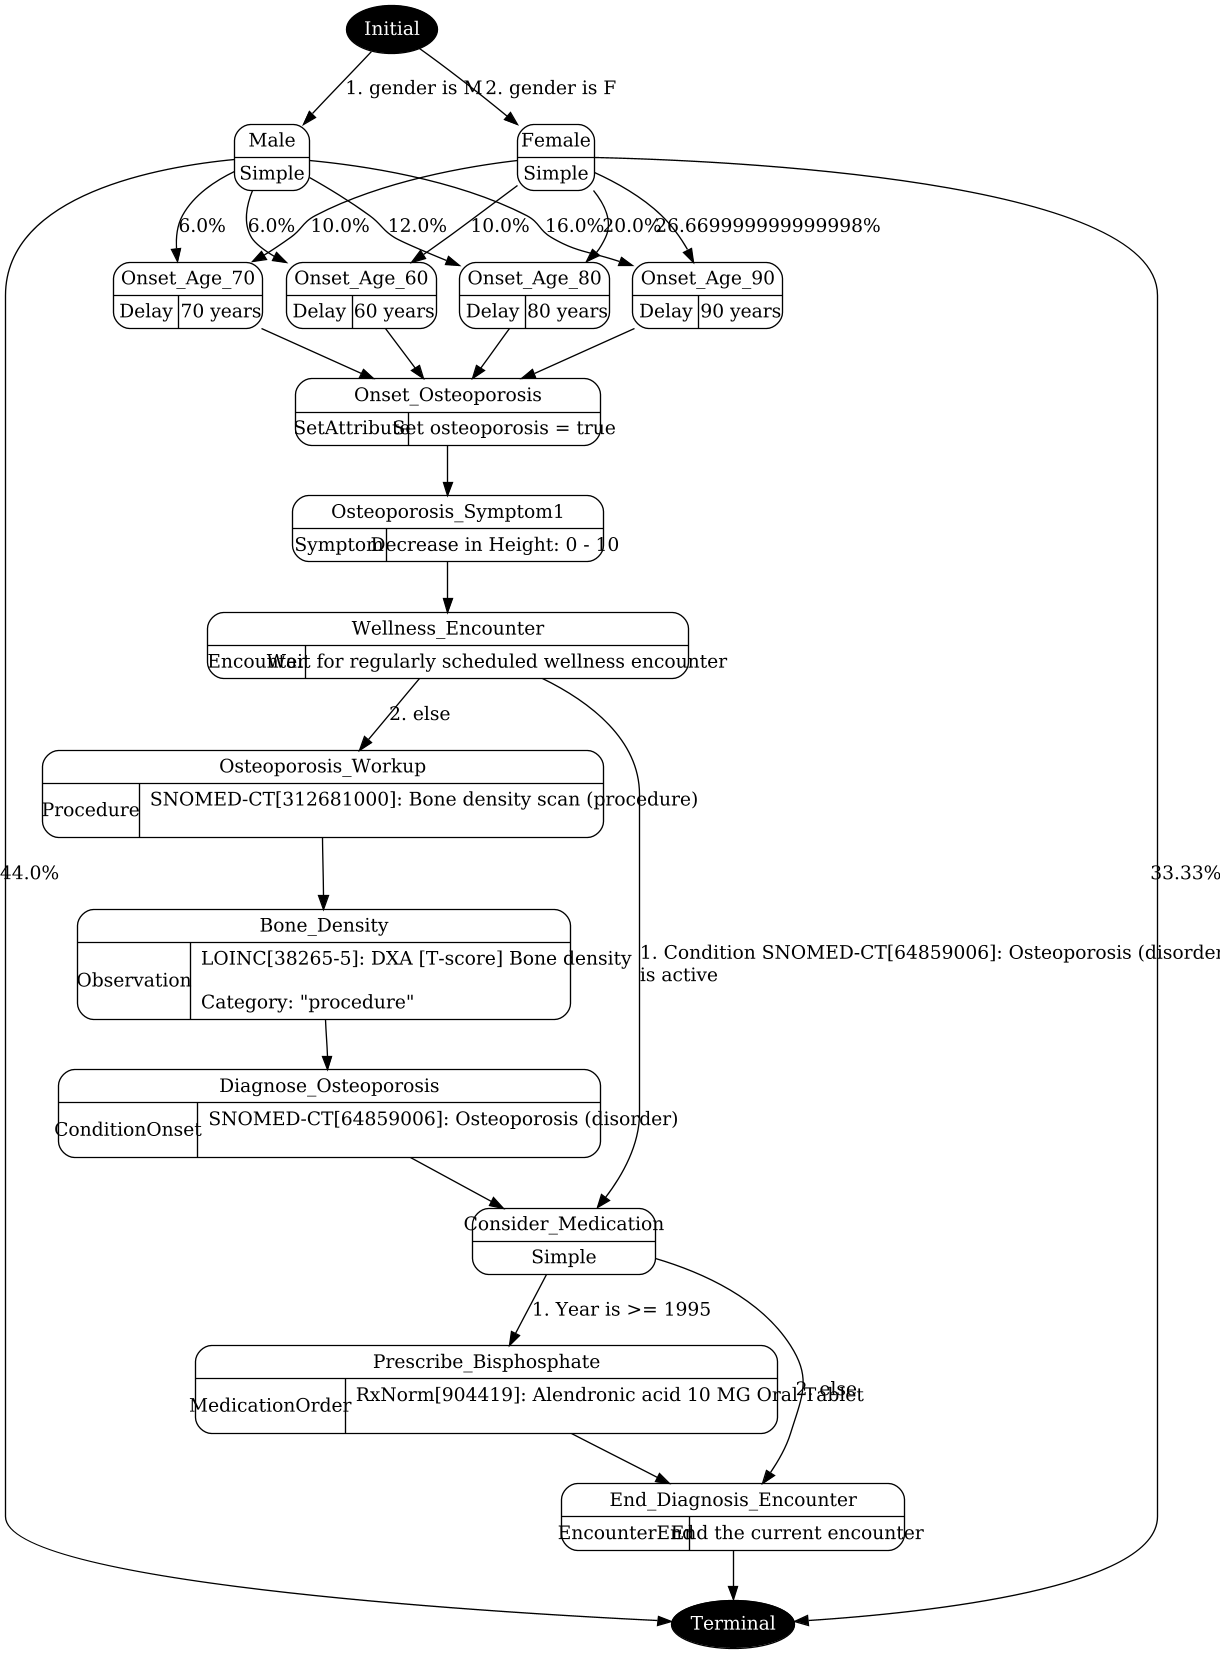
\includegraphics[width=1.0\textwidth]{assets/osteoporosis.png}
	\caption{Synthea Osteoporose Modul \cite{26}}
	\label{fig:osteoporose}
\end{figure} 
\begin{landscape}
\begin{figure}[htbp]
	\caption{Synthea Knochenbruch Bayes-Netz}
	\label{synthea-brokenbone}
	\centering
\begin{tikzpicture}[
	node distance=1cm and 1cm,
	mynode/.style={draw,ellipse,text width=2cm,align=center}
	]
	\node[mynode] (Osteoporosis) {Osteoporosis};
	\node[above= of Osteoporosis] (empty) {};
	\node[mynode,left = of Osteoporosis] (brokenbone) {Broken bone};
	\node[mynode, below right = of Osteoporosis] (brokenhip) {Broken hip};
	\node[mynode, below = of brokenhip] (brokenclavicle) {Broken clavicle};
	\node[mynode, left = of brokenclavicle] (brokenrib) {Broken rib};
	\node[mynode, left = of brokenrib] (brokenwrist) {Broken wrist};
	\node[mynode, left = of brokenwrist] (brokenankle) {Broken ankle};
	\node[mynode, above = of brokenankle](brokenarm) {Broken arm};
	\path [-latex]
	(empty) edge (Osteoporosis)
	(Osteoporosis) edge(brokenarm)
	(Osteoporosis) edge(brokenwrist)
	(Osteoporosis) edge(brokenankle)
	(Osteoporosis) edge(brokenrib)
	(Osteoporosis) edge(brokenclavicle)
	(Osteoporosis) edge(brokenhip)
	(brokenbone) edge(brokenarm)
	(brokenbone) edge(brokenwrist)
	(brokenbone) edge(brokenankle)
	(brokenbone) edge(brokenrib)
	(brokenbone) edge(brokenclavicle)
	(brokenbone) edge(brokenhip);
	\node[above=0.4cm of brokenarm]
	{
		\begin{tabular}{|c|c|c|}
			\hline
			\multicolumn{3}{|c|}{broken arm} \\
			$BB$ & $O$ & $P(BA \mid BB,O)$  \\
			\hline
			T & T & $0.417$ \\
			T & F & $0.225$ \\
			\hline
		\end{tabular}
	};
	\node[below=0.4cm of brokenankle]
	{
		\begin{tabular}{|c|c|c|}
			\hline
			\multicolumn{3}{|c|}{broken ankle} \\
			$BB$ & $O$ & $P(BA \mid BB,O)$  \\
			\hline
			T & T & $0.101$ \\
			T & F & $0.2$ \\
			\hline
		\end{tabular}
	};
	\node[below=0.4cm of brokenwrist]
	{
		\begin{tabular}{|c|c|c|}
			\hline
			\multicolumn{3}{|c|}{broken wrist} \\
			$BB$ & $O$ & $P(BW \mid BB,O)$  \\
\hline
			T & T & $0.101$ \\
			T & F & $0.2$ \\
			\hline
		\end{tabular}
	};
	\node[below=0.5cm of brokenrib]
	{
		\begin{tabular}{|c|c|c|}
			\hline
			\multicolumn{3}{|c|}{broken rib} \\
			$BB$ & $O$ & $P(BR \mid BB,O)$  \\
\hline
			T & T & $0.05$ \\
			T & F & $0.1$ \\
			\hline
		\end{tabular}
	};
	\node[below=0.4cm of brokenclavicle]
	{
		\begin{tabular}{|c|c|c|}
			\hline
			\multicolumn{3}{|c|}{broken clavicle} \\
			$BB$ & $O$ & $P(BC \mid BB,O)$  \\
\hline
			T & T & $0.101$ \\
			T & F & $0.225$ \\
			\hline
		\end{tabular}
	};
	\node[above=2.1cm of brokenhip]
	{
		\begin{tabular}{|c|c|c|}
			\hline
			\multicolumn{3}{|c|}{broken hip} \\
			$BB$ & $O$ & $P(BH \mid BB,O)$  \\
\hline
			T & T & $0.23$ \\
			T & F & $0.05$ \\
			\hline
		\end{tabular}
	};
	\node[above=0.4cm of brokenbone]
{
	\begin{tabular}{|c|c|c|}
		\hline
		broken bone \\
		$P(BB)$  \\
		\hline
		$14,061$\\
		\hline
	\end{tabular}
};

\end{tikzpicture}
\end{figure}
\end{landscape}



\chapter{Auswertungen der medizinischen Datenbanken }\label{chap:Auswertung}
In diesem Kapitel wird die Sicherheit von Angerona an einem praxisnahen Anwendungsfall gezeigt. Dafür wird zuerst geprüft, ob der definierte Schwellwert eingehalten wird,f indem aus dem Vorwissen des Angreifermodells der Schwellwert berechnet wird. Anschließend wird gezeigt, dass bei einem größer definierten Schwellwert als das Vorwissen, der Zugriff verweigert wird. Andersherum wird gezeigt, dass bei kleiner definiertem Schwellwert als das Vorwissen, der Zugriff gewährt wird.\\  Anschließend wird gezeigt, dass mithilfe der Historie erkannt wird, ob beim Zulassen einer Anfrage eine Sicherheitsregel verletzt werden würde. \\ Um die Laufzeit zu messen, wird die Laufzeitmessung aus der Arbeit von Angerona genauer betrachtet und mit unseren Hardwarespezifikationen gemessen. Dann werden mit Synthea zwei verschieden große, synthetische, medizinischen Datenbanken generiert und  für das einfache Osteoporose-Beispiel und für das komplexere Knochenbruch-Beispiel geprüft, wie sich die Laufzeiten bei verschieden komplexen Abhängigkeiten verhalten. Anschließend wird die Laufzeit von den medizinischen Datenbanken MIMIC-III und eICU bei wachsender Anzahl von Sicherheitsregeln getestet und geschaut, wie sich die Laufzeit dabei verhält. \\ \\
Die Datenbanken und der Server auf dem Angerona ausgeführt wird, laufen auf einer virtuellen Maschine in einem PowerEdge R530 Server. Dieser Server hat zwei Intel Xeon E5-2620 v3 Prozessoren 2,4GHz mit jeweils 6 Core / 12 Threads und 64GB DDR4-SDRAM. Als Datenbanksystem wird PostgreSQL mit der Version 9.5.24 verwendet. \\ 

\section{Sicherheit}
\subsection{Schwellwert}\label{sub:schwellwert}
Betrachtet wird im Folgenden das Beispiel aus \autoref{chap:Beispiel}. Um zu prüfen, ob der Schwellwert eingehalten wird, wird das Beispiel vereinfacht. Es wird im Angreifermodell das Vorwissen, dafür das Alice Eltern Krebs haben, von Mallory für Alice (id 1) auf 100\% gesetzt. Dies wird umgesetzt, indem die Variablen $p\_vaterhatkrebs$ und $p\_mutterhatkrebs$ auf $1/1$ gesetzt werden, wie in \autoref{code-mallorysvorwissen} zu sehen ist.
\begin{Pseudocode}[caption={Mallorys Vorwissen}, label={code-mallorysvorwissen}]
1/1 :: p_patient(1).
25/100 :: p_raucher(1).
1/1 :: p_mutterhatkrebs(1).
1/1 :: p_vaterhatkrebs(1).
\end{Pseudocode}
Anschließend kann der Schwellwert berechnet werden, indem für jede mögliche Klausel \textit{krebs(X)}, die noch eintreffen kann, die Wahrscheinlichkeiten aufaddiert werden. Diese ist in dem Fall folgende, weil nur noch die Abhängigkeit \enquote{Raucher} variabel ist:
\begin{itemize}
	\item[$\bullet$] \texttt{krebs(X) :- patient(X), raucher(X), mutterhatkrebs(X), vaterhatkrebs(X), v1111(X).}
	\item[\bullet] \texttt{krebs(X) :- patient(X), NOT raucher(X), mutterhatkrebs(X), vaterhatkrebs(X), v1011(X).}
\end{itemize}
Somit ist der Schwellwert für $krebs(X) = (\frac{1}{1} \cdot \frac{25}{100} \cdot \frac{1}{1} \cdot \frac{1}{1} \cdot \frac{6}{10}) + (\frac{1}{1} \cdot 1- \frac{25}{100} \cdot \frac{1}{1} \cdot \frac{1}{1} \cdot \frac{35}{100}) = \frac{33}{80} $. \\  Nun kann die Sicherheitsregel für krebs(X) für Mallory auf den Schwellwert gesetzt werden und es wird als Ergebnis von Angerona \textit{true} ausgegeben, da auf den Wert zugegriffen werden darf, wie in \autoref{code-thresholdAccess} zu sehen ist. Allerdings wird bei einem Schwellwert $ > \frac{33}{80}$ der Zugriff verweigert, wie im \autoref{code-thresholdNoAccess} zu sehen ist. 


\begin{Pseudocode}[caption={Angerona Ergebnis für Schwellwert=$\frac{33}{80}$}, label={code-thresholdAccess}]
Write a command. Write 'Stop' to conclude.
AS mallory:krebs('1')
ACCESS CONTROL RESULT
	Acc.Ctrl.: true
ACTION RESULT
	Result: true Exception: false
\end{Pseudocode}

\begin{Pseudocode}[caption={Angerona Ergebnis für Schwellwert=$\frac{34}{80}$}, label={code-thresholdNoAccess}]
Write a command. Write 'Stop' to conclude.
AS mallory:krebs('1')
ACCESS CONTROL RESULT
	Acc.Ctrl.: false Cause: mallory : krebs ('1') is not authorized
\end{Pseudocode}

Damit wurde gezeigt, dass Angerona den Schwellwert richtig berechnet und den Zugriff erfolgreich verweigert, wenn das Vorwissen größer dem Schwellwert ist.

\subsection{Temporäre Historie}
Im Folgenden wird das Beispiel von \cref{sub:schwellwert} fortgesetzt. Es wird geprüft, ob Angerona bei einer Anfrage erkennt, ob durch die Genehmigung der Antwort eine andere Sicherheitsrichtlinie verletzt wird. Dafür erstellt Angerona eine temporäre Historie während der Ausführung, in der die Historie um die Anfrage erweitert wird und prüft anschließend ob durch die temporäre Historie eine Sicherheitsregel verletzt wird. \\ 
Um zu prüfen, ob die temporäre Historie ein solchen Fall erkennt, wird in Angerona die Anfrage gestellt, ob Alice eine Raucherin ist. Aber da die Information dafür, dass Alice Raucherin ist, den Schwellwert auf $\frac{6}{10}$ anhebt und somit das Vorwissen $\geq$ Schwellwert ist, wird der Zugriff verweigert, wie in \autoref{code-history} zu sehen ist. 

\begin{Pseudocode}[caption={Angerona Ergebnis für die Abfrage, ob Alice Raucherin ist}, label={code-history}]
Write a command. Write 'Stop' to conclude.
AS mallory:raucher('1')
ACCESS CONTROL RESULT
	Acc.Ctrl.: false Cause: mallory : raucher ('1') is not authorized
\end{Pseudocode}

\section{Laufzeit}
Die Messung der Laufzeit wird in Online- und Offlinelaufzeit unterteilt. Die Onlinelaufzeit beschreibt die Zeit, die vergeht, zwischen dem Stellen einer Anfrage und dem Erhalten des Ergebnisses der Anfrage. Die Offlinelaufzeit beschreibt die Zeit zwischen dem Start von Angerona bis zu dem Zeitpunkt an dem Angerona bereit für eine Eingabe ist. \\ 
Dabei ist bei der Onlinelaufzeit besonders wichtig, dass diese nicht zu hoch ist, da sonst die Benutzer lange Wartezeiten  für jede Anfrage haben. Die Offlinelaufzeit hingegen kann auch länger dauern, da Angerona in der Praxis nur einmal gestartet wird.  \\
Jedoch ist bereits beim Start der kleineren medizinischen Datenbank MIMIC-III die Offlinelaufzeit nach 24 Stunden zu keinem Ende gekommen. Deshalb wird im ersten Schritt mit Synthea getestet, wie groß eine Patientendatenbank werden kann, sodass diese noch in angemessener Zeit nutzbar ist.   
Anschließend wird gezeigt, wie Angerona sich bei wachsender Anzahl von Sicherheitsregeln verhält.\\ 
Dabei ist jede Onlinelaufzeit das \texttt{worst-case} Szenario und bedeutet, dass der Schwellwert auf 0 gesetzt wird, damit die Überprüfung der Sicherheitsregel bis zum Schluss ausgeführt wird, die Anfrage nicht verweigert und somit abgebrochen wird. Es wurden dabei nicht wie im Paper nur 100 Sicherheitsregeln definiert, sondern jeweils immer für alle Patienten versucht, weil dies praxisnäher ist um die Sicherheit zu gewährleisten. Wenn nur die Patienten abgesichert werden, die zum Beispiel Krebs haben, dann könnte ein Angreifer ohne Historie für alle Patienten abfragen, ob diese Krebs haben und würde nur \texttt{false} oder \texttt{security exceptions} erhalten. Wenn der Angreifer dann durch statistische Recherche herausfindet, dass das Verhältnis der Anzahl der erhaltenen \texttt{security exceptions} zu der bei den \texttt{false} erhalten wurde ca. der Wahrscheinlichkeit entspricht, dass ein beliebiger Patient Krebs hat, kann der Angreifer daraus schließen, dass die Patienten für die eine \texttt{security exception} ausgegeben wurde mit einer sehr hohen Wahrscheinlichkeit Krebs haben bzw. vielleicht sogar alle Krebs haben. \\ 
Jedoch kann dies umgangen werden, indem einigen Patienten, die kein Krebs haben, auch eine Sicherheitsrichtlinie hinzugefügt wird, da dann der Angreifer alle möglichen Ergebnisse erhalten kann. Deshalb sollte mindestens für die Leute die Krebs haben eine Sicherheitsrichtlinie definiert werden, aber es ist von Vorteil noch mehr Sicherheitsregeln zu definieren.

\subsection{Vorhandene Auswertungen}
Die Laufzeit von Angerona wurde bereits in der Arbeit von Guarnieri et. al. \cite{guarnieri2017securing} analysiert. Dabei wurde ein synthetisches \texttt{beliefProgram.pbl} für 1,000 bis 100,000 Patienten generiert, wovon ein Beispiel für 1 Patienten in \autoref{code:cancerExample} zu sehen ist. Davon wurden 100 Patienten mit Sicherheitsregeln abgesichert und anschließend zufällig 100 Anfragen gestellt. \\ 
\begin{Pseudocode}[caption={\texttt{beliefProgram.pbl} für das Beispiel aus \cite{6}}, label={code:cancerExample}]]
cancer(X) :- patient(X), sw1(X).
cancer(X) :- smokes(X), sw2(X).
cancer(Y) :- father(X,Y), mother(Z,Y), cancer(X), NOT cancer(Z), sw3(Y).
cancer(Y) :- father(X,Y), mother(Z,Y), NOT cancer(X), cancer(Z), sw3(Y).
cancer(Y) :- father(X,Y), mother(Z,Y), cancer(X), cancer(Z), sw3(Y), sw4(Y).
cancer(Y) :- father(X,Y), mother(Z,Y), cancer(X), cancer(Z), NOT sw3(Y), sw4(Y).
1/1 :: patient(0).
1/20 :: sw1(0).
5/19 :: sw2(0).
3/14 :: sw3(0).
3/7 :: sw4(0).
\end{Pseudocode}
Das Ergebnis für die Onlinelaufzeit von Guarnieri et. al. \cite{guarnieri2017securing} wird in \autoref{fig:paperlaufzeit} dargestellt. Das Experiment wird für dieselbe Modellierung, aber unseren Hardware Spezifikationen vom Server wiederholt und eine graphische Modellierung des Ergebnisses für die Onlinelaufzeiten ist in \autoref{fig:unserelaufzeit} zu sehen. Die Onlinelaufzeiten unterscheiden sich dabei nicht sehr stark, da diese bei unter 1 Sekunde bleibt bei beliebiger Größe der Datenbank bis 100,000 Patienten. \\
Die Offlinelaufzeit hingegen unterscheidet sich minimal zu der angegebenen aus der Arbeit von Guarnieri et. al. \cite{guarnieri2017securing}, in der eine Maximale-Offlinelaufzeit von 2,5 Minuten für beliebig große Datenbanken bis 100,000 Patienten gemessen wurde. Nach meinen Messungen wächst die Offlinelaufzeit bei wenig definierten Sicherheitsregeln linear und hat bei einer Implementierung für 100,000 Patienten eine Offlinelaufzeit von fast 11 Minuten. Dies kann den Grund haben, dass bei meinen Messungen die Initialisierung von Angerona anhand der 3 Dateien \texttt{beliefProgram.pbl}, \texttt{initStatements.txt} und \texttt{template.cpt} geschieht und diese noch von Angerona eingelesen und die Daten an die Datenbank gesendet werden müssen. In dem Beispiel aus der Arbeit von Guarnieri et. al. \cite{guarnieri2017securing} hingegen wurden die Beispiele direkt in den Code eingebaut, wodurch der Übersetzungsschritt der 3 Dateien wegfällt.\\  
	\begin{figure}[ht]
	\begin{minipage}{.5\textwidth}
		\centering
		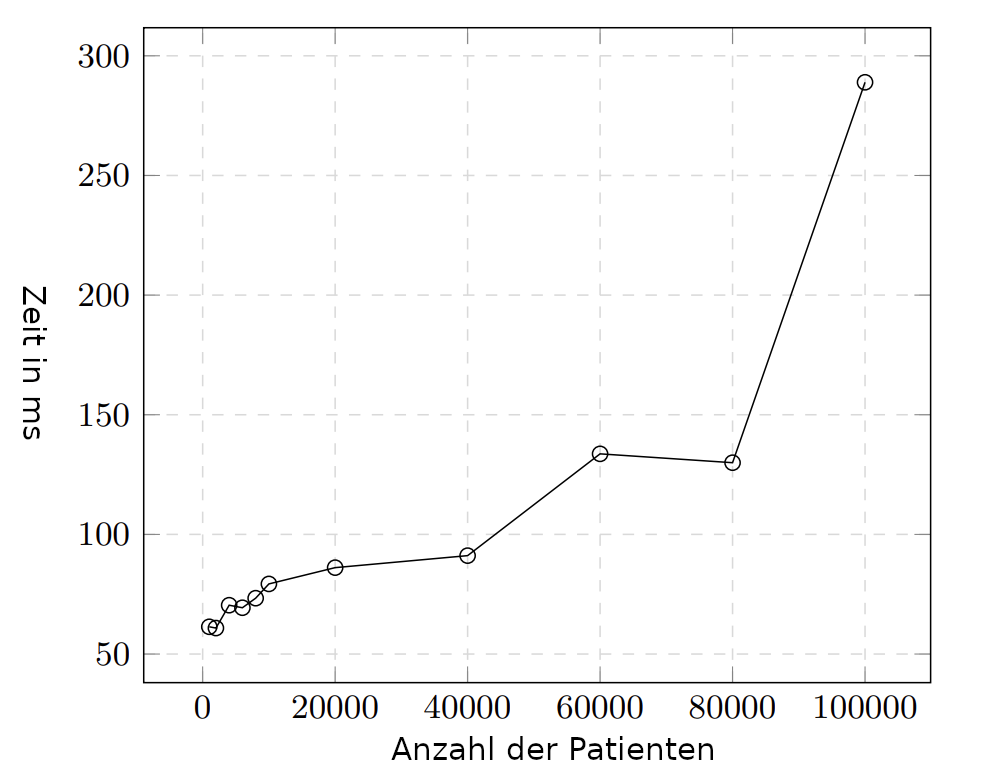
\includegraphics[width=0.9\linewidth]{assets/paperLaufzeit.PNG}
		\caption{Onlinelaufzeit aus \cite{guarnieri2017securing}}
		\label{fig:paperlaufzeit}
	\end{minipage}
	\begin{minipage}{.5\textwidth}
		\centering
		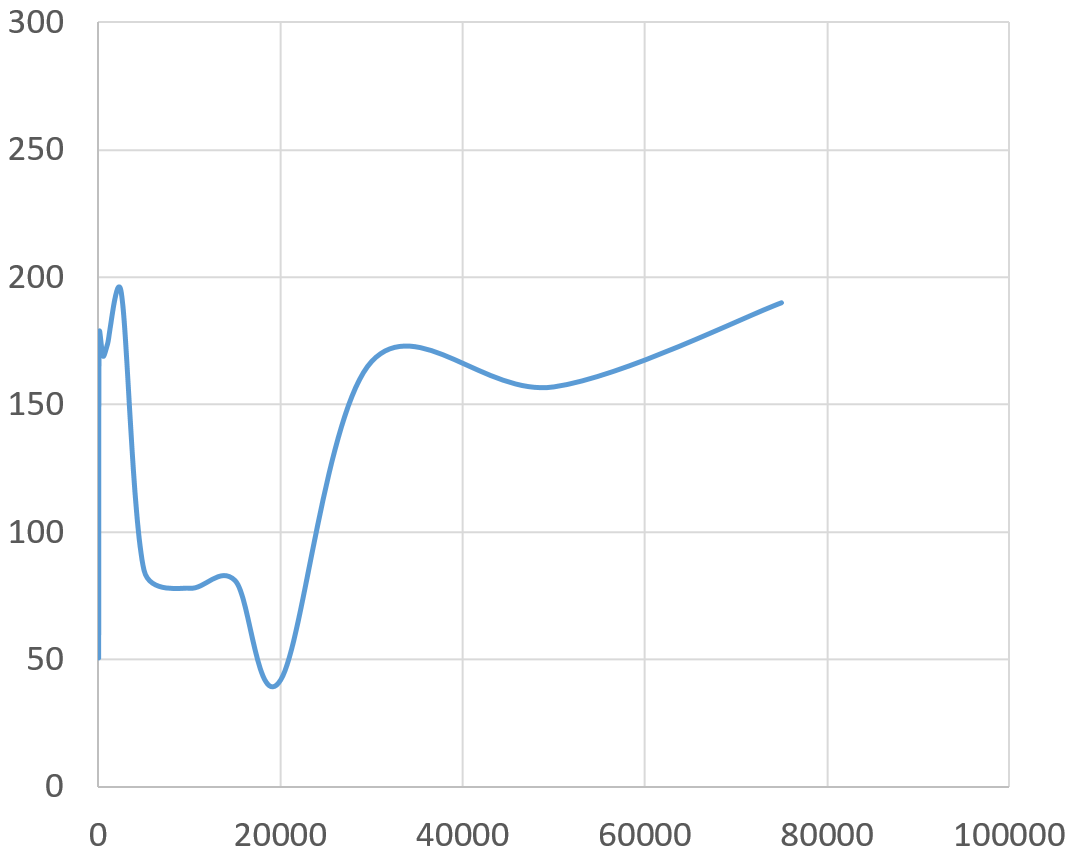
\includegraphics[width=0.9\linewidth]{assets/onlineSkript.png}
		\caption{Onlinelaufzeit Osteoporose}
		\label{fig:unserelaufzeit}
	\end{minipage}
\end{figure}

\subsection{Komplexität des Angreifermodell}
Um zu prüfen, wie Angeronas Laufzeit sich verhält bei wachsender Komplexität der Abhängigkeiten, wird das Osteoporose- und Knochenbruch-Beispiel aus der Synthea Datenbank in Angerona modelliert. Dafür wurden für das Osteoporose-Beispiel für alle Patienten eine Sicherheitsregel für die Abfrage nach der Krankheit Osteoporose mit einem Schwellwert von 0 festgelegt, damit der \emph{worstcase} der Onlinelaufzeit betrachtet wird. Für das Knochenbruch-Beispiel wurde für jeden Patienten alle Arten von Knochenbrüche abgesichert. Eine graphische Modellierung für den Vergleich der Offlinelaufzeit ist in \autoref{fig:syntheaoffline} und der Onlinelaufzeit in \autoref{fig:syntheaonline} zu sehen.\\  Dabei wächst für kleinere Datenbankgrößen die Laufzeit kaum und wird erst bei einer Datenbankgröße mit 3000 Patienten bemerkbar, da hierbei die Differenz der Onlinelaufzeit vom Knochenbruch-Beispiel ca. 750 Millisekunden länger ist und die Offlinelaufzeit ca. 12 Minuten länger als beim Osteoporose-Beispiel. Die Differenz der Komplexität steigt jedoch für komplexere Datenbanken konstant mit, sodass bereits bei einer Datenbankgröße mit 5000 Patienten die Differenz der Offlinelaufzeit 23 Minuten und die Onlinelaufzeitdifferenz 6 Sekunden beträgt.
Gründe für die erhöhten Laufzeiten beim Knochenbruch-Beispiel sind dabei, dass Daten in die Datenbank eingefügt werden, die Angreifermodellierung komplexer und somit die \texttt{beliefProgram.pbl} größer ist und dass es mehr Abhängigkeiten gibt und somit mehr probabilistische Fakten je Patient modelliert werden.  
	\begin{figure}[ht]
		\begin{minipage}{.5\textwidth}
		\centering
		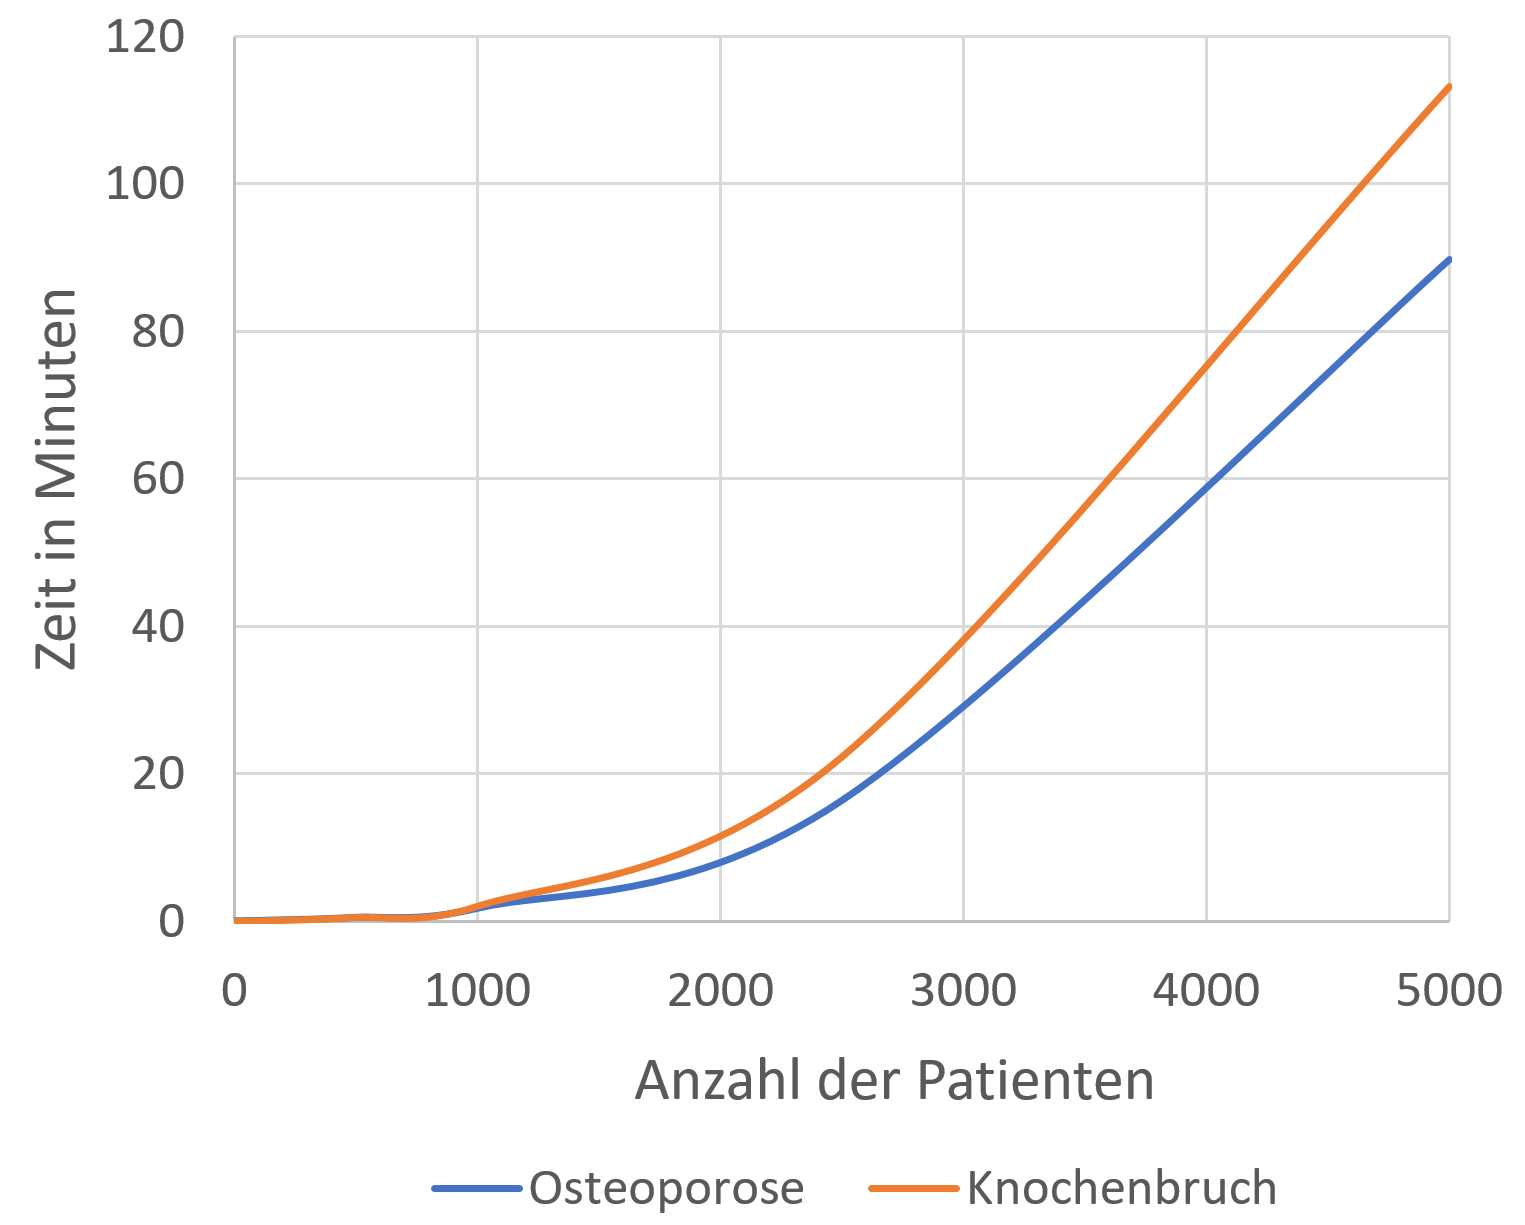
\includegraphics[width=0.9\linewidth]{assets/OfflinezeitSynthea.png}
		\caption{Offlinelaufzeiten Synthea}
		\label{fig:syntheaoffline}
	\end{minipage}
	\begin{minipage}{.5\textwidth}
		\centering
		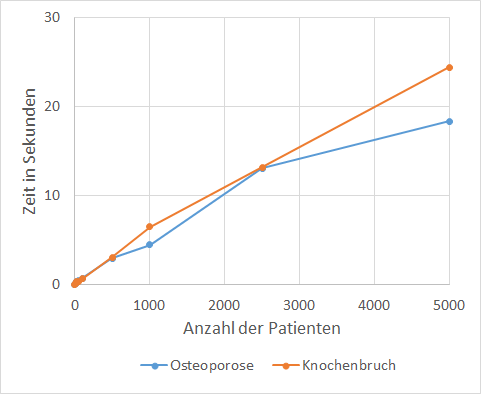
\includegraphics[width=0.9\linewidth]{assets/onlineSynthea.png}
		\caption{Onlinelaufzeiten Synthea}
		\label{fig:syntheaonline}
	\end{minipage}
\end{figure}
\noindent


\subsection{MIMIC-III und eICU bei wachsenden Sicherheitsregeln}
Die MIMIC-III und eICU Datenbank lässt sich nur in Angerona starten, wenn man die Sicherheitsregeln nur für die Patienten definiert, die Krebs haben. Wenn für alle Patienten einen Sicherheitsrichtlinie definiert werden soll, überschreitet die Offlinelaufzeit bereits 24 Stunden und lässt sich somit nicht ausführen. Deshalb wird im Folgenden geprüft, wie sich die \emph{Online- und Offlinelaufzeiten} verhalten bei wachsenden Sicherheitsregeln für die Information, dass ein Patient Krebs hat. Zum Schluss wird die Laufzeit gezeigt, wenn man das Vorwissen des Angreifers und die Sicherheitsregeln nur für Patienten mit Krebs definiert.
Um zu testen wie Angerona sich bei wachsender Größe des Angreifermodells verhält, wird die MIMIC-III und eICU Datenbank verwendet. Dabei werden jeweils für die Datenbanken die Sicherheitsregeln für die Patienten in der \texttt{initStatements.txt} und das Vorwissen in der \texttt{beliefProgram.pbl} erweitert. Dadurch ergeben sich die Onlinelaufzeiten in \autoref{fig:onlinesecures} und die \emph{Offlinelaufzeiten} in \autoref{fig:offlinesecures} . \\ 
Auffällig ist, dass beim eICU-und MIMIC-III-Beispiel die Offlinelaufzeiten annähernd gleich steigen, jedoch verschiedene Startzeiten bei nur einer definierten  Sicherheitsrichtlinie haben. Dies ist dadurch zu erklären, dass initial die benötigte Datenbank generiert wird und diese beim eICU-Beispiel fast vier mal größer ist, als beim MIMIC-III-Beispiel. Die Offlinelaufzeit ist jedoch bei nur einer definierten Sicherheitsrichtlinie nicht vier mal länger für MIMIC-III, da zum Start ist die Offlinelaufzeit für eICU mit $48.8$ Minuten knapp 8 mal länger als für das MIMIC-III-Beispiel mit einer Offlinelaufzeit von ca. $6.5$ Minuten. Der Faktor verringert sich jedoch bei wachsender Anzahl der Sicherheitsregeln und ist bereits bei 10,000 definierten Sicherheitsregeln nur noch knapp 2 mal länger mit einer Offlinelaufzeit für eICU von ca. $105$ Minuten und für MIMIC-III mit $65$ Minuten. \\ 
Die Onlinelaufzeit wächst dabei für MIMIC-III und eICU annähernd linear mit der Anzahl der Sicherheitsregeln, wobei für größere Datenbanken wie bei eICU die Onlinelaufzeit generell etwas höher liegt. Zwar ist bei bis zu 1000 Sicherheitsregeln die Laufzeit identisch und bleibt bei unter 3 Sekunden für beide Fälle, jedoch ab 2000 Sicherheitsregeln ist die Laufzeit für größere Datenbanken (eICU) länger als für kleinere Datenbanken (MIMIC-III). Der Unterschied der Onlinelaufzeit bleibt jedoch annähernd konstant und ist zum Beispiel für die viermal größere Datenbank eICU ca. 4 Sekunden länger als für die MIMIC-III-Datenbank. 
	\begin{figure}[ht]
	\begin{minipage}{.5\textwidth}
		\centering
		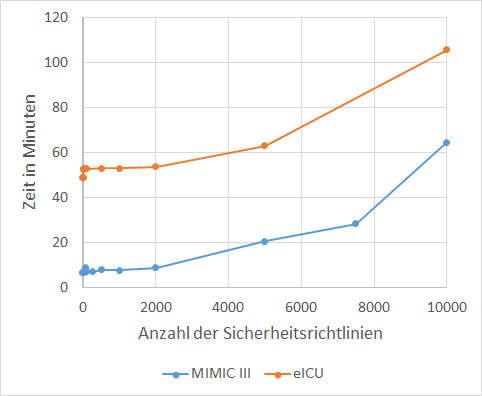
\includegraphics[width=0.9\linewidth]{assets/OfflineEicuMimic.png}
		\caption{Offlinelaufzeiten Sicherheitsregeln}
		\label{fig:offlinesecures}
	\end{minipage}
	\begin{minipage}{.5\textwidth}
		\centering
		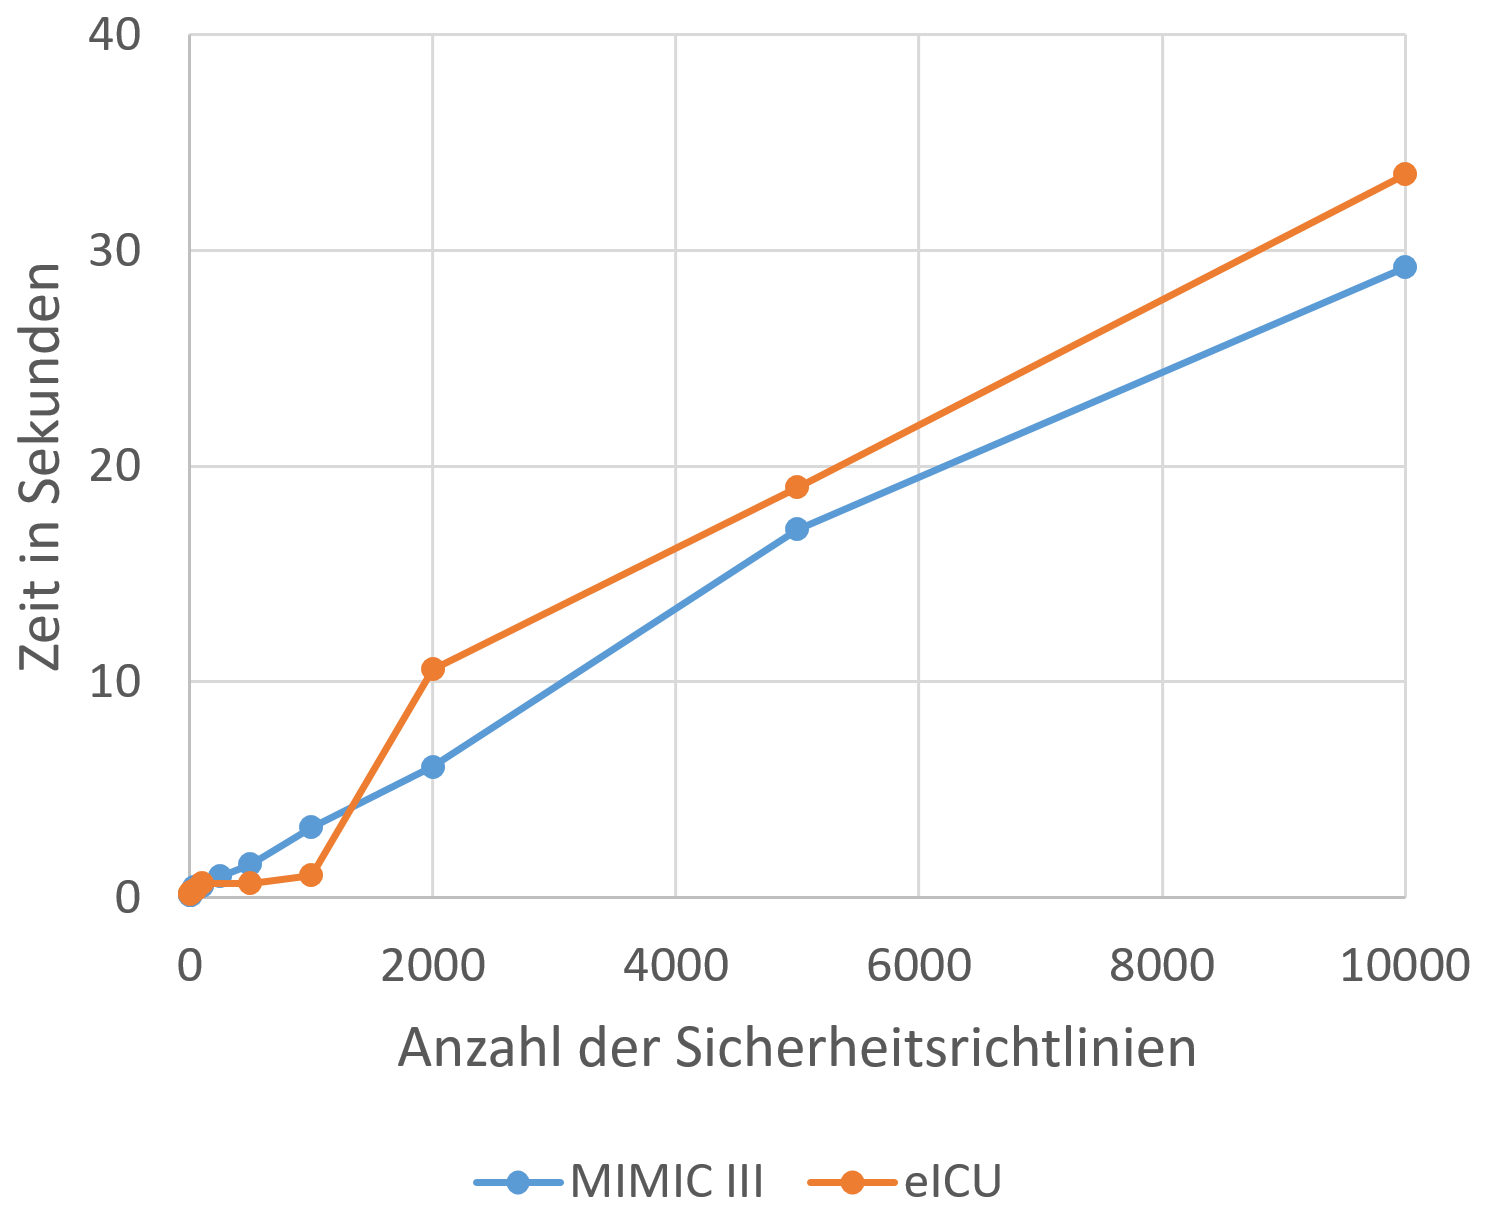
\includegraphics[width=0.9\linewidth]{assets/onlineEicuMimic.png}
		\caption{Onlinelaufzeiten Sicherheitsregeln}
		\label{fig:onlinesecures}
	\end{minipage}
\end{figure}
Für das MIMIC-III-Beispiel wurde außerdem beim Absichern aller Patienten, die Krebs haben, was eine Menge von $13658$ Sicherheitsregeln entspricht, eine Offlinelaufzeit von $77$ Minuten und eine Onlinelaufzeit von $36.4$ Sekunden gemessen. Außerdem ist dabei aufgefallen, dass während Angerona läuft $6.7$ GB vom Arbeitsspeicher reserviert wurde. \\ 
Für das eICU-Beispiel wurde beim Absichern aller Patienten die Krebs haben, was eine Menge von $8179$ Sicherheitsregeln entspricht, eine Offlinelaufzeit von $89$ Minuten und eine Onlinelaufzeit von $23.6$ Sekunden gemessen. Außerdem ist dabei aufgefallen, dass während Angerona läuft $5.8$ GB vom Arbeitsspeicher reserviert wurde. \\ 
Hierbei sieht man, dass die Datenbankgröße, also die Größe der \texttt{initStatements.txt} eher eine Auswirkung auf die Offlinelaufzeit und die Anzahl der Sicherheitsregeln, also die Größe der \texttt{beliefProgram.pbl}, auf die Onlinelaufzeit hat. \\ \\ 
Das Ergebnis der Evaluierung aus Guarnieri et. al. \cite{guarnieri2017securing} wurde unter angepassten Voraussetzung für Angerona getestet, wodurch die positive Laufzeit zustande kam. Wie man in den Auswertung dieser Arbeit sieht, ist die Nutzung von Angerona in realen Anwendungsfällen nicht möglich, weil die Offlinelaufzeiten und Onlinelaufzeiten zu hoch sind. Meiner Meinung nach wäre eine Offlinelaufzeit von maximal 30 Minuten und eine Onlinelaufzeit von maximal 5000 Millisekunden akzeptabel um solch ein System in einem realen Anwendungsfall nutzen zu können. Damit wäre Angerona bei einer Datenbankgröße mit bis zu 100.000 Patienten, nicht zu komplexen Abhängigkeitsregeln und ca. 1000 definierten Sicherheitsregeln effizient nutzbar. Diese Größen reichen für die meisten realen Anwendungsfälle jedoch nicht aus. \\ 
Ein weiteres Problem ist, dass bei jeder Datenbankänderung einer von Angerona abgesicherten Datenbank, die \texttt{initStatements.txt} neu generiert bzw. um die geänderten Werte ergänzt werden muss. Dadurch muss Angerona komplett neu gestartet werden und solange ist die Datenbank, für die Dauer der Offlinelaufzeit, nicht erreichbar. Da dies der Fall ist, ist selbst eine Offlinelaufzeit von 30 Minuten zu hoch und dürfte meiner Meinung nach 5 Minuten nicht überschreiten. \\ Unter diesen Bedingungen würde Angerona in kaum einem realen Anwendungsfall nutzbar sein, da selbst eine kleine Datenbank, wie MIMIC-III, nicht in einer effizienten Offlinelaufzeit Nutzbar wären. \\ 
Des weiteren wurde im Synthea Beispiel festgestellt, dass nur ganze Zahlen für die IDs der Patienten erlaubt sind und somit standardisierte IDs wie die  Universally Unique Identifier (UUID), welche aus Buchstaben, Nummern und Sonderzeichen besteht, nicht von Angerona akzeptiert werden. \\ 

\chapter{Zusammenfassung und Ausblick} \label{chap:Zusammenfassung}
In dieser Arbeit wurde der Prototyp Angerona in ein praxisnahem Anwendungsfall angewendet und evaluiert. Dabei wurde festgestellt, dass die definierten Schwellwerte für die Sicherheitsregeln von Angerona wie spezifiziert eingehalten wurden. Außerdem wird die Sicherheit für die Historie ebenfalls eingehalten, da Angerona erfolgreich prüft, ob eine Anfrage eine Sicherheitsrichtlinie verletzten würde, wenn diese genehmigt werden würde und fügt diese somit der Historie nicht hinzu. \\
Angerona bietet jedoch für praxisnahe Anwendungsfälle keine ausreichende Laufzeit, weil die Onlinelaufzeit bereits für die kleinere Datenbank MIMIC-III mit $36.4$ Sekunden zu hoch ist. Dies liegt daran, dass Angeronas Laufzeit stark durch die Anzahl der definierten Sicherheitsregeln und der dazugehörigen Angreifermodellierung für jeden Krankenhausaufenthalt beeinflusst wird. Ein anderer Faktor, der die Laufzeit beeinflusst, ist die Komplexität der definierten Abhängigkeiten im Angreifermodell. Diese haben einen großen Einfluss auf die Laufzeit, welche bei wachsender Datenbankgröße, eine immer länger Laufzeit aufweist, wie am Synthea-Beispiel gezeigt wurde. \\ 
Hinzu kommt, dass in der Praxis meist noch komplexere Modellierungen abgesichert werden müssen, wenn zum Beispiel noch mehr als nur eine Krankheit abgesichert werden soll. Wenn man davon ausgeht, dass alle Patienten mit allen Krankheiten abgesichert werden sollen, dann würde es nicht möglich sein, dies mit Angerona umzusetzen, weil die Laufzeit zu hoch und der belegte Arbeitsspeicher sehr hoch wäre.
Jedoch wurde in  Guarnieri et. al. \cite{guarnieri2017securing} bereits erwähnt, dass die Laufzeit durch Parallelisierung verbessert werden kann, da Angerona alle Berechnungen auf einem Kern durchführt. Deshalb ist der Prototyp Angerona eine gute Grundlage, um diesen zu verbessern oder um sich für weitere Entwicklungen von DBIC-Mechanismen inspirieren zu lassen. \\ 
Eine Erweiterung, die das Laufzeitverhalten ebenfalls beeinflussen könnte, wäre ein Gruppensystem für die Definition der probabilistischen Abhängigkeitsregeln, sodass es möglich ist, das Vorwissen für mehrere Patienten gleichzeitig zu definieren. Außerdem wäre eine bessere Ausgabe von Fehlermeldungen hilfreich beim Interagieren mit Angerona, da Angerona sich bei falschen Anfragen beendet und unklare Fehlermeldungen auswirft. \\ \\ 
Die Laufzeit liegt, wie in \cref{sub:bayes} erwähnt, laut Guarnieri et. al. \cite{guarnieri2017securing} in \texttt{PTIME}, unter der Voraussetzung, dass das Bayes-Netz die Eingeschaften eines Polytrees erfüllt. Jedoch wäre es auch hilfreich, wenn Angerona auch die Bedingung etwas einschränken könnte, wie im Knochenbruch-Beispiel von Sythea erwähnt wurde, dass die Bedingung \enquote{Knochenbruch} eigentlich auch von \enquote{Osteoporose} Abhängig ist, aber leider nicht auf die Art modelliert werden kann. Daher wäre es in manchen realen Anwendungsfällen sinnvoll, würde Angerona ein Bayes-Netz ohne Polytree Eigenschaften akzeptieren. \\ 
Eine zukünftige Erweiterungen für Angerona wäre auch, wenn Angerona Bayes-Netze als Eingabe für die Angreifermodellierung akzeptieren würde und somit übersichtlich ein Angreifermodell erstellt werden kann, dass direkt in ein Angerona konformes Schema übersetzt wird.





% Normally, the bibliography comes next at this point. Do *not* (try
% to) include further indices and tables like an index or
% a list of figures or a list of tables or such things. Nobody 
% actually uses them and they just use up space. 
%
% You *can* however include a glossary, if this seems appropriate. It
% goes here as an unnumbered chapter. Most thesis will *not* need a
% glossary: a well-written text (re)explains strange words and
% concepts as necessary. However, there are situations where a
% glossary may be helpful.














%%%
% 
% Bibliographies
%
%%%
%
% The uzl-thesis class will load biblatex for the bibliography
% management. This is a powerful package, see its documentation for
% details. The styles will be setup correctly and automatically by
% choosing one of the two style keys as described earlier.
%
% In order for the bibliography to work, run latex in the following
% order (which is the standard order):
% 
% > lualatex thesis-example
% > bibtex thesis-example
% > lualatex thesis-example
% 
% Add BibTeX files using \addbibresource or use the {bibtex entries}
% environment (see below).
%
%%%
%
% Although everyting is normally setup automatically, you can change
% the options passed to biblatex using the key 'biblatex';
% for instance,
%
%   \UzLThesisSetup{biblatex={firstinits=false}}
%
% will switch off shortened first names. Normally, you will not need
% this key in your preamble. 
% 
% Note that the bibtex program is used as the 'backend' of biblatex
% by default (rather than biber, which is the preferred program of
% biblatex). This means that you can (and must) run *bibtex* after you
% have run lualatex on your thesis. If you wish to use biber instead
% of bibtex, say 'biblatex={backend=biber}'. 
% 
%%%
%
% The following environment is optional. It allows you to keep the
% bibtex entries for your thesis right here in the thesis file. What
% happens is that each time this tex file is processed, the contents
% of the following environment gets written to the file
% \jobname-bibtex-entries.bib (this file gets overwritten each
% time). Independently, \addbibresource{\jobname-bibtex-entries.bib}
% is always called if the file \jobname-bibtex-entries.bib
% exists. 
%
% In result, you can edit and keep the bibliography's bibtex entries
% right here. If you change something here, run latex, then bibtex,
% then latex once more.
%
% If you would like to manage the bibtex entries in a separate file,
% remove the below environment, delete the \jobname-bibtex-entries.bib
% file and instead write
%
% \addbibresource{filename-of-your-bibtex-file.bib}
%
% in the preamble.
%
%%%


% !!!!!!!!!!!!!!!!!!!!!!!!!!!!!!!!!!
% !!! Your action is needed here !!!
% !!!!!!!!!!!!!!!!!!!!!!!!!!!!!!!!!!
%
% Replace following example entries with the ones of your thesis.



% If you need to have an appendix (I advise against it), insert it
% here using, first, \appendix and then \chapter and then,
% possibly, \section. 
%
% \appendix
%
% \chapter{Technical Appendix}
%
% \section{Experimental Parameters} % possibly
%
% Again, I advise against using an appendix.


\end{document}

%  LocalWords:  LaTeX tex moretexcs Lübeck pdf uzl lualatex bibtex th
%  LocalWords:  TechReport Kernighan Lamport's Tantau's Tantau cls kZ
%  LocalWords:  Mustermann emacs oldschool pdflatex texmf utf biber
%  LocalWords:  biblatex Alphabetische Bibliographie Numerische VIIa
%  LocalWords:  varioref german Einleitung Beiträge dieser Arbeit xml
%  LocalWords:  Ergebnisse Verwandte Arbeiten Aufbau nucleotide VIIc
%  LocalWords:  ensembl amino phylogenetic Alexa Siri decrypt versa
%  LocalWords:  cryptographic pre nondeterministic deterministically
%  LocalWords:  Beutelspacher Untersuchungen zum genetischen sep llcc
%  LocalWords:  Beispiel tikz jpg png Alegrya Kasimir Malewitsch PGF
%  LocalWords:  Lamport Institut für Theoretische Informatik zu url
%  LocalWords:  Universität Springer DowneyF Downey Parameterized doi
%  LocalWords:  BibLaTeX Kime Philipp urldate Mittelbach hyperref Lua
%  LocalWords:  Rahtz Oberdiek Heiko Braams Bezos López fontspec Das
%  LocalWords:  Arseneau amsmath ist Tipps und zur Formulierung
%  LocalWords:  mathematischer Gedanken Mathematik Studienanfänger
%  LocalWords:  Albrecht Vieweg Teubner Verlag
